\chapter{Measurement of \bmumu Branching Fractions}
\label{sec:BFanalysis}
This chapter presents the measurements of the \bdmumu and \bsmumu branching fractions. Section~\ref{sec:BFAnalysisStrategy} gives an overview of the analysis strategy and a description of how the number for \bmumu decays is extracted from the data is given in Section~\ref{sec:signalPdfs}. The estimation of the background decays present in that data set is detailed in Section~\ref{sec:backgrounds}. The normalisation procedure to convert the number of observed \bmumu decays in to the branching fractions for these decays is explained in Section~\ref{sec:Normalisation} and the results are presented in Section ~\ref{sec:BFResults}. 

The work presented in this Chapter was performed by the \bmumu LHCb analysis group and is published here~\cite{}. My contribution was providing the ROOT files which contained the data and simulated events necessary for the analysis development and results and maintaining the stripping selection used for this analysis.

\section{Analysis Strategy} 
\label{sec:BFAnalysisStrategy}
The \bmumu branching fractions, $\mathcal{B}$(\bmumu), are defined as the ratio of \bmumu decays that occur to the number of \bsd mesons created. However in reality not every \bmumu decay occurring will be within the LHCb detector acceptance, get reconstructed and pass the selection criteria of Chapter~\ref{selection_chapter}. Therefore the number of observed \bmumu decays at LHCb is reduced from the number of \bmumu decays occurring by the efficiency, $\epsilon$, of the detector, reconstruction and selection.
The \bmumu branching fractions can be given by
\begin{equation}
\mathcal{B}(B^{0}_{(s)} \to \mu^{+} \mu^{-}) = \frac{\mathcal{N}_{B^{0}_{(s)} \to \mu^{+} \mu^{-}}}{\mathcal{N}_{B^{0}_{(s)}}} = \frac{\mathcal{N}^{obs}_{B^{0}_{(s)} \to \mu^{+} \mu^{-}}}{\eplison \mathcal{N}_{B^{0}_{(s)}}}
\label{eq:BFdef}
\end{equation}
where $\mathcal{N}_{B^{0}{(s)} \to \mu^{+} \mu^{-}(B^{0}_{(s)})}$ is the total number of \bmumu decays (\bsd mesons) and $\mathcal{N}^{obs}_{B^{0}_{(s)} \to \mu^{+} \mu^{-}}$ the number of observed \bmumu decays.


The number of \bsd created can be calculated from the integrated luminosity, $\mathcal{L}_{int}$, and the \bbbar production cross-section, $\sigma_{b \bar{b}}}$, via
\begin{equation}
\mathcal{N}_{B^{0}_{(s)}} = 2 \times \mathcal{L}_{int} \times \sigma_{b \bar{b}} \times f_{d(s)} 
\label{eq:NumberB}
\end{equation}

where $f_{d(s)}$ is the hadronisation factor giving the probability for a $b$ or $\bar{b}$ quark to form a \bd (\bs) or a $\bar{B^{0}}$ ($\bar{B^{0}_{s}}$). The factor of 2 arises because no distinction is made between the \bsd and the $\bar{B^{0}_{s}}$. Although the number of \bsd can be computed this way the measured cross-section is not precisely known. Therefore to achieve a more precise branching fraction measurement an alternative approach is used. Another decay with a well know branching fraction is used to normalise the observed number of \bmumu decays and obtain the branching fractions. The extraction of $\mathcal{B}$(\bmumu) from the number of observed decays therefore is done using
\begin{equation}
\begin{split}
\mathcal{B}(B^{0}_{(s)} \to \mu^{+} \mu^{-}) &= \frac{1}{\mathcal{B}_{norm}} \cdot \frac{f_{norm}}{f_{d(s)}} \cdot \frac{\epsilon_{norm}}{\epsilon_{B^{0}_{(s)} \to \mu^{+} \mu^{-}}} \cdot \frac{\mathcal{N}^{obs}_{B^{0}_{(s)} \to \mu^{+} \mu^{-}}}{\mathcal{N}^{obs}_{norm}} \\
&= \alpha_{d(s)} \cdot \mathcal{N}_{obs}_{B^{0}_{(s)} \to \mu^{+} \mu^{-}}
\end{split}
\label{eq:BFnorm}
\end{equation}
where $norm$ indicates the normalisation channel. The normalisation parameters can be combined into one normalisation parameter $\alpha_{d(s)}$ for each of the \bs and \bd decays. The normalisation procedure removes the uncertainty from $\sigma_{b \bar{b}}$. Therefore the number of observed \bmumu decays and the normalisation parameters, $\alpha_{d(s)}$, need to be evaluated to measure the branching fractions. The selection described in Chapter~\ref{selection_chapter} allows \bmumu candidates to be classified by their dimuon invariant mass and global BDT output. %As illustrated in Figure~\ref{}. 
A simultaneous unbinned maximum likelihood fit is performed to the dimuon invariant mass distribution in 4 BDT bins to measure the observed number of \bdmumu and \bsmumu decays. The Run 1 and Run 2 data are kept separate and the fit is applied simultaneously to both data sets. To measure the number of \bmumu decays the fit requires knowledge of the mass shapes and the fraction of \bmumu decays in each BDT bin and the number of background decays and their mass shapes in each bin. The mass shapes and fraction of \bmumu decay in each BDT bin are described by probability density functions (\pdfs). The evaluation of the \bmumu mass \pdfs and the fraction of decays in each BDT bin are described in Section~\ref{sec:signalPdfs}. The expected number of background decays and their mass \pdfs in each BDT bin are described in Section~\ref{sec:backgrounds}.  


The binning choice used for the BDT is chosen to optimise both fit stability and sensitivity to the \bmumu branching fractions. The bin boundaries used are
\begin{equation}
[0.25, 0.4, 0.5, 0.6, 1.0].
\label{eq:BDTbins}
\end{equation}
Candidates with BDT values between 0 and 0.25 are not included in the fit because this bin is dominated by backgrounds from combinatorial decays. The inclusion of this bin does not improve the branching fraction sensitivity and reduces the stability of the fit. %The highest BDT is the largest due to the excellent performance of the BDT at removing background decays. Table/Figure X, shows the number of \bmumu candidates in data passing the selection described in Chapter X with dimuon mass greater that 5447 \mevcc. At high BDT values there are very few candidated therefore a wide bin is used for high BDT values to ensure there are enough candidates in high mass regions to ensure a stable, accurate fit.

The normalisation decay can be chosen to be as similar as possible to \bmumu decays to reduce systematic uncertainties introduced by different detection and selection efficiencies. Furthermore the chosen decay needs to be abundant so the the precision of the \bmumu branching fraction measurements are not limited by the statistics available for the normalisation channel and it must have a precisely measured branching fraction, which is likely for abundant decays. Two decays are chose as normalisation channels; \bujpsik where \jpsimumu and \bdkpi. Both decays have large, precisely measured branching fractions and are similar to \bmumu decays in complementary ways. The \bujpsik decay has a very similar trigger efficiency to \bmumu decays due to the two muons from the \jpsi but the extra particle, the $K^{+}$ in the final state leads to different selection and reconstruction efficiencies. The \bdkpi decay has a very similar topology to \bmumu therefore the selection and reconstruction efficiencies will be similar, but the trigger efficiencies for hadrons is quite different compared to muons.  

The normalisation factors $\alpha_{d(s)}$ for \bdmumu and \bsmumu decays are evaluated independently for each normalisation channel and year of data taking, the factors are combined to produce an overall normalisation factor for Run 1 and Run 2. The evaluation of the normalisation factors is described in Section~\ref{sec:Normalisation}.



\section{\bsmumu mass and BDT \pdfs}
\label{sec:signalPdfs}

\subsection{Mass \pdfs}
The mass \pdfs for \bdmumu and \bsmumu decays are modelled by a Crystal Ball function~\cite{Skwarnicki:1986xj}. A Crystal Ball function is a Gaussian function that has an exponential tail on the low mass side to model radiative energy loss in the the final state. The parameters defining the function are the mean, $\mu$, and resolution, $\sigma$ of the Gaussian, the slope of the exponential, $n$, and a parameter $\alpha$, defined in terms of $\sigma$, that determines the transition point between the Gaussian and the exponential function. 

The parameters are evaluated using different methods:
\begin{itemize}
\item $\mu$ - the mean for \bd and \bs are evaluated separately from a fits to \bdkpi and \bskk decays in data
\item $\sigma$ - the resolution is extrapolated from the resolutions of quarkonia resonances. The resolutions for the \jpsi, $\Psi (2S)$ and $\Upsilon(1, 2, 3S)$ decaying into two muons are measured from a fits to data. The \bd and \bs resolutions are then extrapolated from the observed relationship between quarkonia mass and resolution.
\item $n$ and $\alpha$ - these parameters are evaluated from the mass spectrum of \bdmumu and \bsmumu simulated decays where the mass distributions are smeared to have the same resolution as that measured from the quarkonia decays in data.
\end{itemize}

All parameters are evaluated separately for the \bd and \bs for each year of data taking. The resulting parameter vales are in good agreement across each year in the Run 1 and Run 2 data sets. The weighted average of the yearly parameters therefore is used to produced the mass \pdfs for Run 1 and Run 2 and are given in Tables~\ref{tab:signalpdfRun1} and~\ref{tab:signalpdfRun2} .
%I am concerned about this table because I do not know where the uncertainties come from ....
\begin{table}[htbp]
\begin{center}
\begin{tabular}{lcc}
 \hline
Parameter & \bdmumu & \bsmumu \\  \hline
$\mu$/\mevcc &5284.73 $\pm$ 0.15_{stat} $\pm$ 0.27_{syst} & 5372.05 $\pm$ 0.16_{stat} $\pm$ 0.36_{syst} \\ 
$\sigma$/\mevcc & 22.68 $\pm$ 0.05_{stat} $\pm$ 0.39_{syst} &23.07 $\pm$ 0.05_{stat} $\pm$ 0.39_{syst}\\
$n$& 1.141 $\pm$ 0.026 & 1.156 $\pm$ 0.013 \\
$\alpha$ & 2.054 $\pm$ 0.013 & 2.053 $\pm$ 0.007 \\  \hline
\end{tabular}
\vspace{0.7cm}
\caption{\bmumu mass \pdf parameter values for Run 1.}
\label{tab:signalpdfRun1}
\end{center}
\end{table}

\begin{table}[htbp]
\begin{center}
\begin{tabular}{lcc}
 \hline
Parameter & \bdmumu & \bsmumu \\  \hline
$\mu$/\mevcc &5279.95 $\pm$ 0.13_{stat} $\pm$ 0.08_{syst} & 5367.34 $\pm$ 0.14_{stat} $\pm$ 0.35_{syst} \\ 
$\sigma$/\mevcc & 22.46 $\pm$ 0.08_{stat} $\pm$ 0.41_{syst} &22.85 $\pm$ 0.08_{stat} $\pm$ 0.42_{syst}\\
$n$& 1.118 $\pm$ 0.014 & 1.110 $\pm$ 0.017 \\
$\alpha$ & 2.063 $\pm$ 0.007 & 2.062 $\pm$ 0.008 \\
 \hline
\end{tabular}
\vspace{0.7cm}
\caption{\bmumu mass \pdf parameter values for Run 2.}
\label{tab:signalpdfRun2}
\end{center}
\end{table}

\subsection{BDT \pdfs}
%The fraction of \bmumu decays in each BDT bin is meeded to measure the branching fraction therefore the BDT \pdf needs to be evaluated. 
The global BDT distribution for \bmumu decays is expected to be uniform between 0 and 1 as designed by the flattening procedure described in Section~\ref{}. The fraction of \bmumu decays in a BDT bin should simply be proportional to the bin with. However the global BDT was trained and flattened using simulated decays therefore to avoid  differences between simulated decays and data affecting the expected fraction of \bmumu decays in each BDT bin, the BDT \pdf is evaluated from data. This process is know as the BDT calibration.
The global BDT is designed to used only kinematic and geometric information to classify candidates and include no PID information. Therefore the BDT distributions of \bhh decays, that are topologically similar to \bmumu decays, will be the same as \bmumu decays. \bdkpi decays are used to calibrate the BDT response because it is the most abundant \bhh decay. 

The number of \bdkpi decays is extracted from data using maximum likelihood fits in each BDT bin for each year of data taking. The \bdkpi candidates must pass the standard \bhh selection in Table~\ref{} and are separated from other \bhh modes using  DLL$_{K\pi}$ variable. To reduce the difference in the trigger efficiency between \bdkip and \bmumu decays, \bdkpi candidates are required to be TIS at the L0 and Hlt1 but TOS at Hlt2 to ensure enough statistics.

The particle identification and trigger efficiencies are different for \bdkpi and \bmumu decays. Therefore the \bdkpi yields in each BDT bin are corrected for using by the different trigger and particle identification efficiencies. The same calibration is used for \bsmumu and \bdmumu decays.
The calibration is preformed for each year separately then combined to give the Run 1 and Run 2 fractions per BDT bin. Figure~\ref{fig:BDTpdfs} shows the BDT distribution for \bmumu decays calibrated with \bdkpi data for Run 1 and Run 2. 

\begin{figure}[htbp]
    \centering
   \begin{subfigure}[b]{0.48\textwidth}
        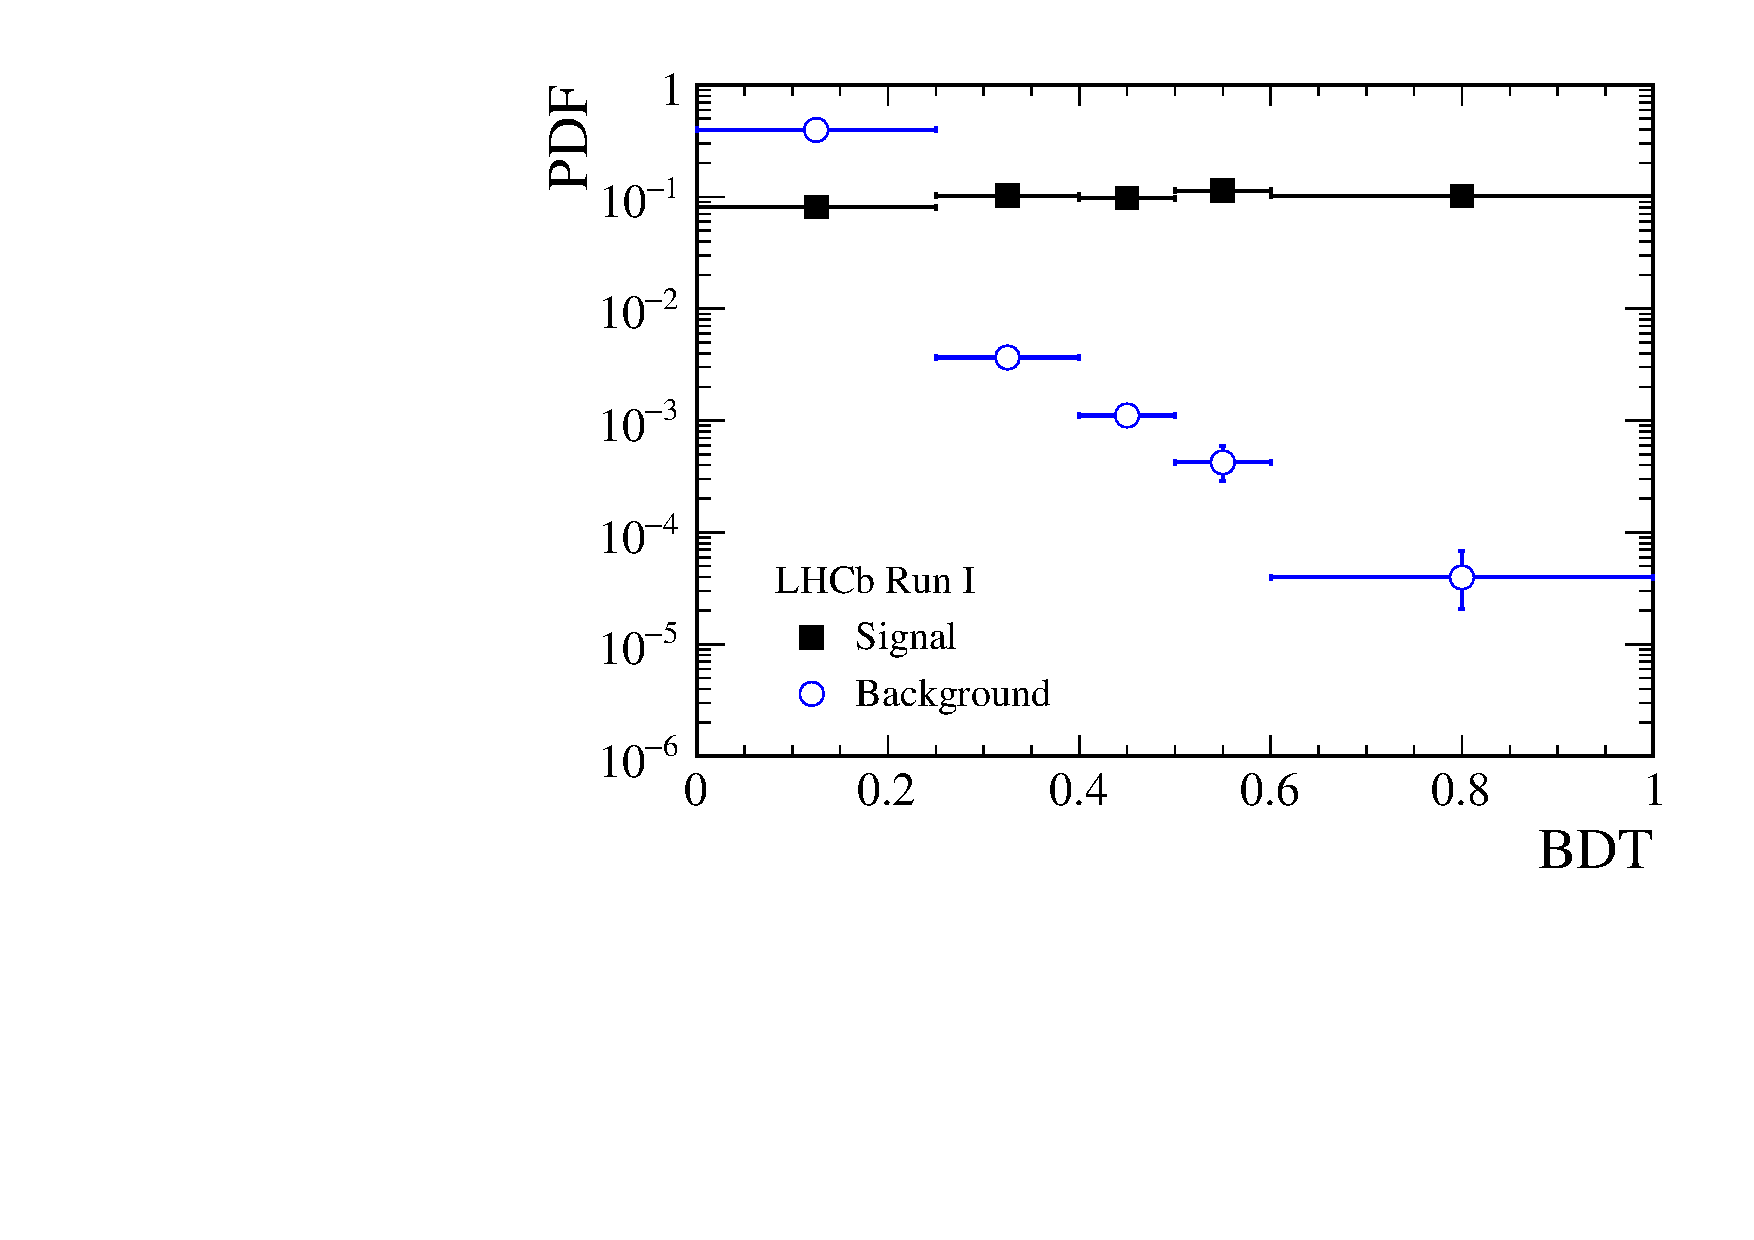
\includegraphics[width= \textwidth]{./Figs/BFAnalysis/C_macros/BDT_calibration_Run1.pdf}
        %\caption{ }
       % \label{fig:BDTSsig}
    \end{subfigure}
   % ~ %add desired spacing between images, e. g. ~, \quad, \qquad, \hfill etc. 
      %(or a blank line to force the subfigure onto a new line)
    \begin{subfigure}[b]{0.48\textwidth}
       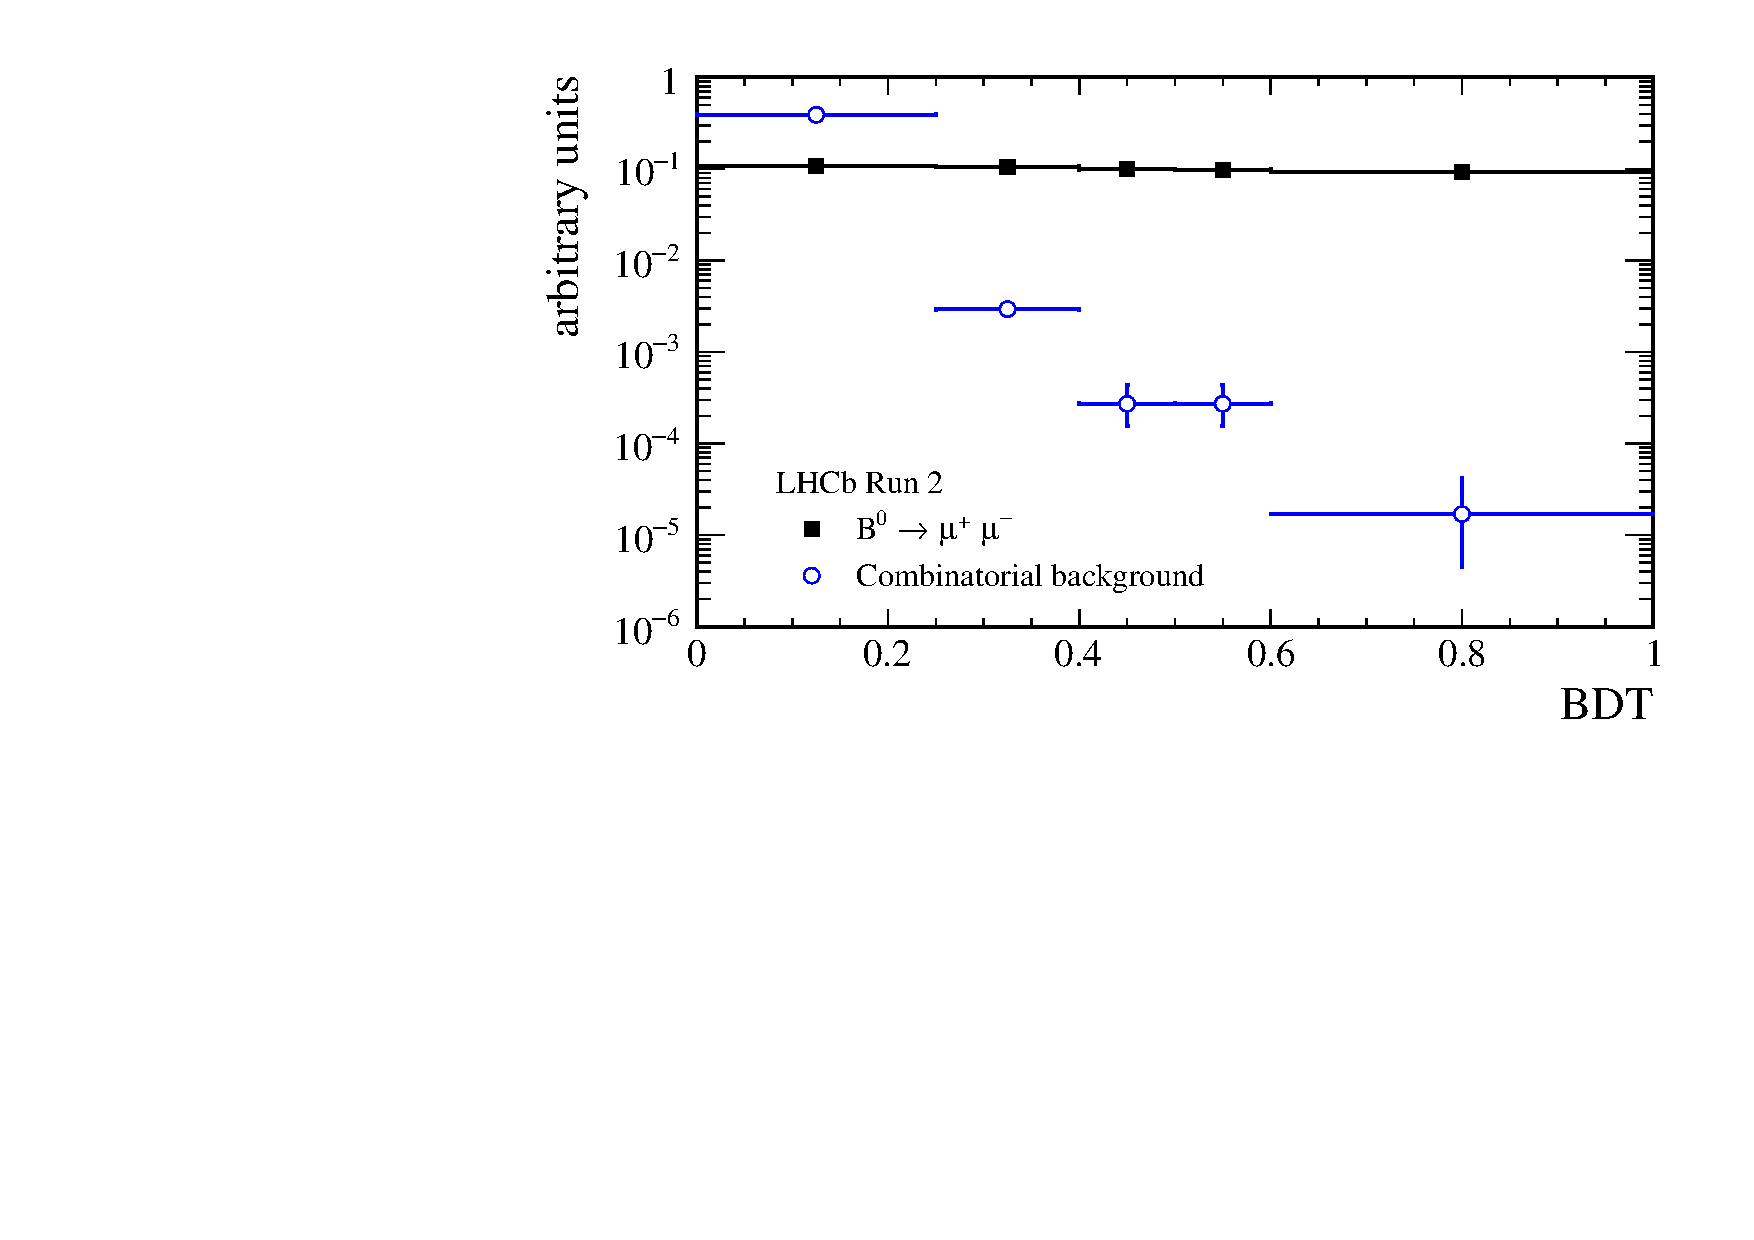
\includegraphics[width=\textwidth]{./Figs/BFAnalysis/C_macros/BDT_calibration_Run2.pdf}
      %  \caption{ }
     %   \label{fig:BDTSbkg}
   \end{subfigure}
    \caption{\bmumu BDT \pdfs (black squares) for Run 1 and Run 2 data calibrated on \bdkpi decay and the combinatorial background decays (blue circles) for \bmumu candidates in data with a dimuon mass above 5477 \mevcc. }
    \label{fig:BDTpdfs}
\end{figure}


\subsection{Decay time dependence of the \bsmumu BDT \pdf}
\label{sec:ADGBDTcorrections}
The output of the global BDT for \bmumu is correlated with the \bmumu decay time due the the choice of input variables used in the BDT as listed in Section~\ref{}. This correlation will lead of slightly incorrect estimations of the \bsmumu BDT \pdf. In the SM the \bsmumu effective lifetime, \tmumu, is equal to the lifetime of the heavy \bs mass eigenstate, \tH, however in reality \tmumu could be somewhere in between the lifetimes of the heavy and light mass eigenstates. As described in Chapter ({\it the Theory Chapter}) the \bsmumu effective lifetime is related to the parameter \ADG, where \ADG = +1 for \tmumu = \tH and \ADG = -1 for \tmumu = \tL, where \tL is the lifetime of the light \bsmumu mass eigenstate.

The simulated decays used to train and flatten the global BDT use as the \bsmumu effective lifetime the mean of the measured \tH and \tL values at the time of production. Therefore the lifetime used is different between simulation versions. Since the BDT output is correlated with the lifetime the BDT \pdf, the fractions of \bsmumu decays in each BDT bin, will depend on the lifetime used in the simulation. Numerical correction factors are computed for each year to scale the BDT \pdf for the situation where \ADF = -1, 0 or +1, so that the dependence on \ADG of the measured branching fractions can be evaluated.

No corrections are needed for \bdmumu because the difference in lifetime of the heavy and light \bd mass eigenstates  is negligible and the need for correction cancels out with the BDT calibration that uses the \bd decay \bdkpi. 

%{\it I have some questions about this part, how are these corrections actually used since the BDT is flattened for Run 1 with 2011 and for Run 2 with 2015 MC.How is the callibration ok since it uses the B0 which has the same correlations which is this not taken into accout? Prehaps make this briefer?}

\section{Background mass \pdfs and expected yields}
\label{sec:backgrounds}
The selection described in Chapter~\ref{selection_chapter} is effective at reducing the background in the data set to a suitable level so that number of the \bmumu decays can be measured. However background decays are present in the final data set, these cannot be completely removed without drastically reducing the efficiency to select signal decays. The backgrounds present in the final data set must be included in the fit to the dimuon invariant mass in order to accurately measure the \bmumu branching fractions. The backgrounds present in the final data set come from;
\begin{itemize}
\item \bhh decays (where h = $K$, $\pi$) when both hadrons are mis-identified as muons because the hadrons decay during their flight through the detector after leaving the VELO. This background falls within the \bd mass window but not the \bs mass window\footnote{\bd and \bs mass windows are defined as $\pm$ 60 \mevcc of the \bd and \bs masses.} due to the missing energy from the undetected neutrino. 
\item semi-leptonic decays where one hadron is mis-identified as a muon that include;
\begin{itemize}
\item \bdpimunu and \bsKmunu decays where the final state hadrons are mis-identified as muons. The mass of these backgrounds falls below the \bd mass window in the left mass sideband
\item \lambdab decays when the proton is mis-identified as a muon. The large mass of the $\Lambda_{d}$ means that this background pollutes the \bs and \bd mass windows and below these windows
\end{itemize}
\item semi-leptonic decays where muon muons in the decay form a good vertex that include;
\begin{itemize}
\item \bpimumu decays where the pion is not detected. The missing hadron means that these backgrounds fall well below the \bd mass window.
\item \bcjpsimunu decays where \jpsimumu. The large mass of the $B^{+}_{c}$ causes this background of cover the full mass range 4900 - 6000 \mevcc
\end{itemize}
\item combinatorial background formed by the random combination of any two muons in the event, this background is distributed across the full mass range
\end{itemize}

%To measure the number of \bsmumu decays these backgrounds must be modelled in the invariant mass fit in each BDT bin, therefore the mass \pdfs and fraction of events present in each BDT bin must be determined.  Backgrounds that fall below the \bd and \bs mass windows still need to be accruatly modelled so that the number of combinatorial background decays that cover the full mass range can be accuratley described/measured. The proceedure is slightly different for \bhh decays compared to semi-leptonic decays.
In the fit to the dimuon invariant mass the combinatorial background is modelled by an exponential function. The combinatorial background yield is not constrained in the fit and the slope is constrained to have the same value across all BDT bins for each data set. These parameters are determined from a fit to candidates in data for in BDT bin in the mass ranges [4900, ($m_{B^{0}} - 50$)] \mevcc and [($m_{B^{0}_{0}$ + 60, 6000] \mevcc, where the mass shapes and yields of the remaining backgrounds are constrained as well.
The mass \pdfs and yields of the background from \bhh and semi-leptonic decays are constrained in the fir around the expected values. The background that have lower masses than the \bd and \bs must be accurately modelled in the fit to ensure that combinatorial background yield, that spans the full mass range, can be accurate described within the signal mass windows. The approaches for finding th mass \pdfs and expected yields differ for \bhh and semi-leptonic backgrounds, these procedures are described in the following sections.

\subsection{\bhh mass and BDT \pdfs}
The mass \pdf describing mis-identified \bhh decays is formed of two Crystal Ball functions. The parameter values are evaluated from simulated decays for \bdkpi, \bskk, \bdpipi and \bskpi the have the momentum of tracks smeared to model the hadrons decaying in flight. The parameters are evaluated separately for each decay and combined using the branching fractions and the particle identification efficiencies for each decay.

The number of mis-identified \bhh decays in each BDT bin, $\mathcal{N}_{B \to hh \to \mu \mu}$, is found using the relationship
\begin{equation}
\mathcal{N}_{B \to hh \to \mu \mu} = \epsilon^{TRIG}_{B^{0}_{(s)} \to \mu^{+} \mu^{-}} \cdot \frac{\mathcal{N}_{B \to hh}}{\epsilon^{TRIG}_{B \to hh}} \cdot \epsilon_{B \to hh \to \mu\mu}  \\
\label{eq:bhhprediction}
\end{equation}
where ${\mathcal{N}_{B \to hh}$ is the number of TIS \bhh decays in data, $\epsilon^{TRIG}_{B^{0}_{(s)} \to \mu^{+} \mu^{-}, B \to hh}$ are the \bmumu and \bhh trigger efficiencies and $ \epsilon_{B \to hh \to \mu\mu}$ is the probability that a \bhh decays is mis-identified as \bmumu. The number of \bhh decays triggered by TIS us calculated for the full BDT range from the number of \bdkpi decays in data corrected for the expected fraction of \bhh decays is mode occupies. Apart form the trigger and particle identification requirements the same selection is used for \bdkpi decays as \bmumu, therefore only the trigger and particle identification efficiencies are corrected for. The efficiencies are calculated using a combination of data and simulated decays for each BDT bin and the same BDT \pdf as \bmumu decays is assumed for \bhh decays. 

%The expected yield of mis-identified \bhh decays in each BDT bin for Run 1 and Run 2 data are given in Table~\ref{}.

\subsection{Semi-leptonic mass and BDT \pdfs}
The mass \pdfs of semi-leptonic backgrounds vary across the BDT range therefore these \pdfs are evaluated using simulated decays separated into each BDT bin. An Argus function~\cite{Argus_pdf} is used to describe the mass distributions. The shapes of \bdpimunu and \bsKmunu are extremely similar and therefore these backgrounds are modelled with one common \pdf. Similarly one mass \pdf is used to model \bpimumu decays.

The expected yield of the semi-leptonic backgrounds in each BDT bin is estimated by normalising to the number of \bujpsik decays observed via

\begin{equation}
%\begin{split}
\mathcal{N}^{exp}_{x} = \mathcal{N}_{B^{+} \to J/\psi K{+}} \cdot \frac{f_{x}}{f_{u}} \cdot \frac{\mathcal{B}_{x}}{\mathcal{B}_{B^{+} \to J/\psi K^{+}}} \cdot \frac{\epsilon_{x}}{\epsilon^{B^{+} \to J/\psi K^{+}}} 
%&= \beta \cdot f_{x} \cdot \epsilon^{tot}_{x} \cdot \mathcal{B}_{x}
%\end{split}
\label{eq:BkgndPredict}
\end{equation}
where $x$ represents each background decay. The background estimation can be factorised as
\begin{equation}
%\begin{split}
\mathcal{N}^{exp}_{x} = \beta \cdot f_{x} \cdot \epsilon_{x} \cdot \mathcal{B}_{x}
%\end{split}
\label{eq:BkgndPredict2}
\end{equation}
where $\beta$ combined the yield, detection and selection efficiency and hadronisation factors of \bujpsik decays and is the same for all backgrounds. The $\beta$ term is evaluated using the same method as the normalisation of the \bmumu branching fractions described in Section~\ref{sec:Normalisation}. The \bujpisk efficiencies and yields aer evaluated across the full BDT range whereas the detection and selection efficiency of each background, $ \epsilon_{x}$, are evaluated separately for each BDT bin from information from both data and simulated decays. The hadronisation factors and branching fractions are specific to each background and were possible measured, rather than predicted, branching fractions are used. %The expected yields of semi-leptonic backgrounds in each BDT bin for Run 1 and Run 2 data are given in Table~\ref{}.

\section{Normalisation}
\label{sec:Normalisation}

As introduced earlier the \bmumu branching fractions are measured by normalising the number of observed\bmumu decays the number of observed \bujpsik and \bdkpi decays. 
The normalisation parameters $\alpha_{d(s)}$, in equation~\ref{eq:BFnorm} for \bmumu decays depend on the yields of the normalisation decays, the ratio of the detection and selection efficiencies and the hadronisation factors. The evaluation of each of these terms are described in the following sections.

%The normaliation paramters, $\apha_{d(s)}$ in equation~\ref{eq:BFnorm} can be re-written in more detail as


%\begin{equation}
%\end{split}
% \alpha_{d(s)} = \frac{1}{\mathcal{B}_{norm}} \cdot \frac{f_{norm}}{f_{d(s)}} \cdot \frac{\epsilon^{ACC}_{norm}}{\epsilon^{ACC}_{B^{0}_{(s)} \to \mu^{+} \mu^{-}}} \cdot \frac{\epsilon^{RECSEL|ACC}_{norm}}{\epsilon^{RECSEL|ACC}_{B^{0}_{(s)} \to \mu^{+} \mu^{-}}} \cdot \frac{\epsil%n^{TRIG|RECSEL}_{norm}}{\epsilon^{TRIG|RECSEL}_{B^{0}_{(s)} \to \mu^{+} \mu^{-}}} \cdot \frac{1}{\mathcal{N}^{obs}_{norm}}
%\end{split}
%\label{eq:BFnormDetailed}
%\end{equation}

%the efficiency term has been split up into several components indicting the efficiency of different stages of event selection.  The evaluations of different terms in equation~\ref{eq:BFnormDetailed} are described in the following sections.


\subsection{\bdkpi and \bujpsik yields}
The yields of \bujpsik and \bdkpi decays, $ \mathcal{N}^{obs}_{norm}$, are calculated from data using maximum likelihood fits to each year of data taking. 
The \bujpsik mass pdf is modelled by an Ipathia function~\cite{} and the fit includes components for combinatorial background and $B^{+} \to J/\psi \pi^{+}$ decays that are mis-reconstructed as \bujpsik. The mass \pdf parameters are determined from both data and simulated decays. The \bdkpi yields are calculated in the same way at the BDT calibration and the same trigger requirements are used. However for the normalisation the total number of \bdkpi decays across the full BDT range is needed rather the bin-by-bin yields. Figure~\ref{fig:Bdkpiyield}~and~\ref{fig:Bujpsikyield} show the mass fits used to calculate the Run 1 and Run 2 \bdkpi and \bujpsik yields.


\begin{figure}[htbp]
    \centering
  \begin{subfigure}[b]{0.48\textwidth}
        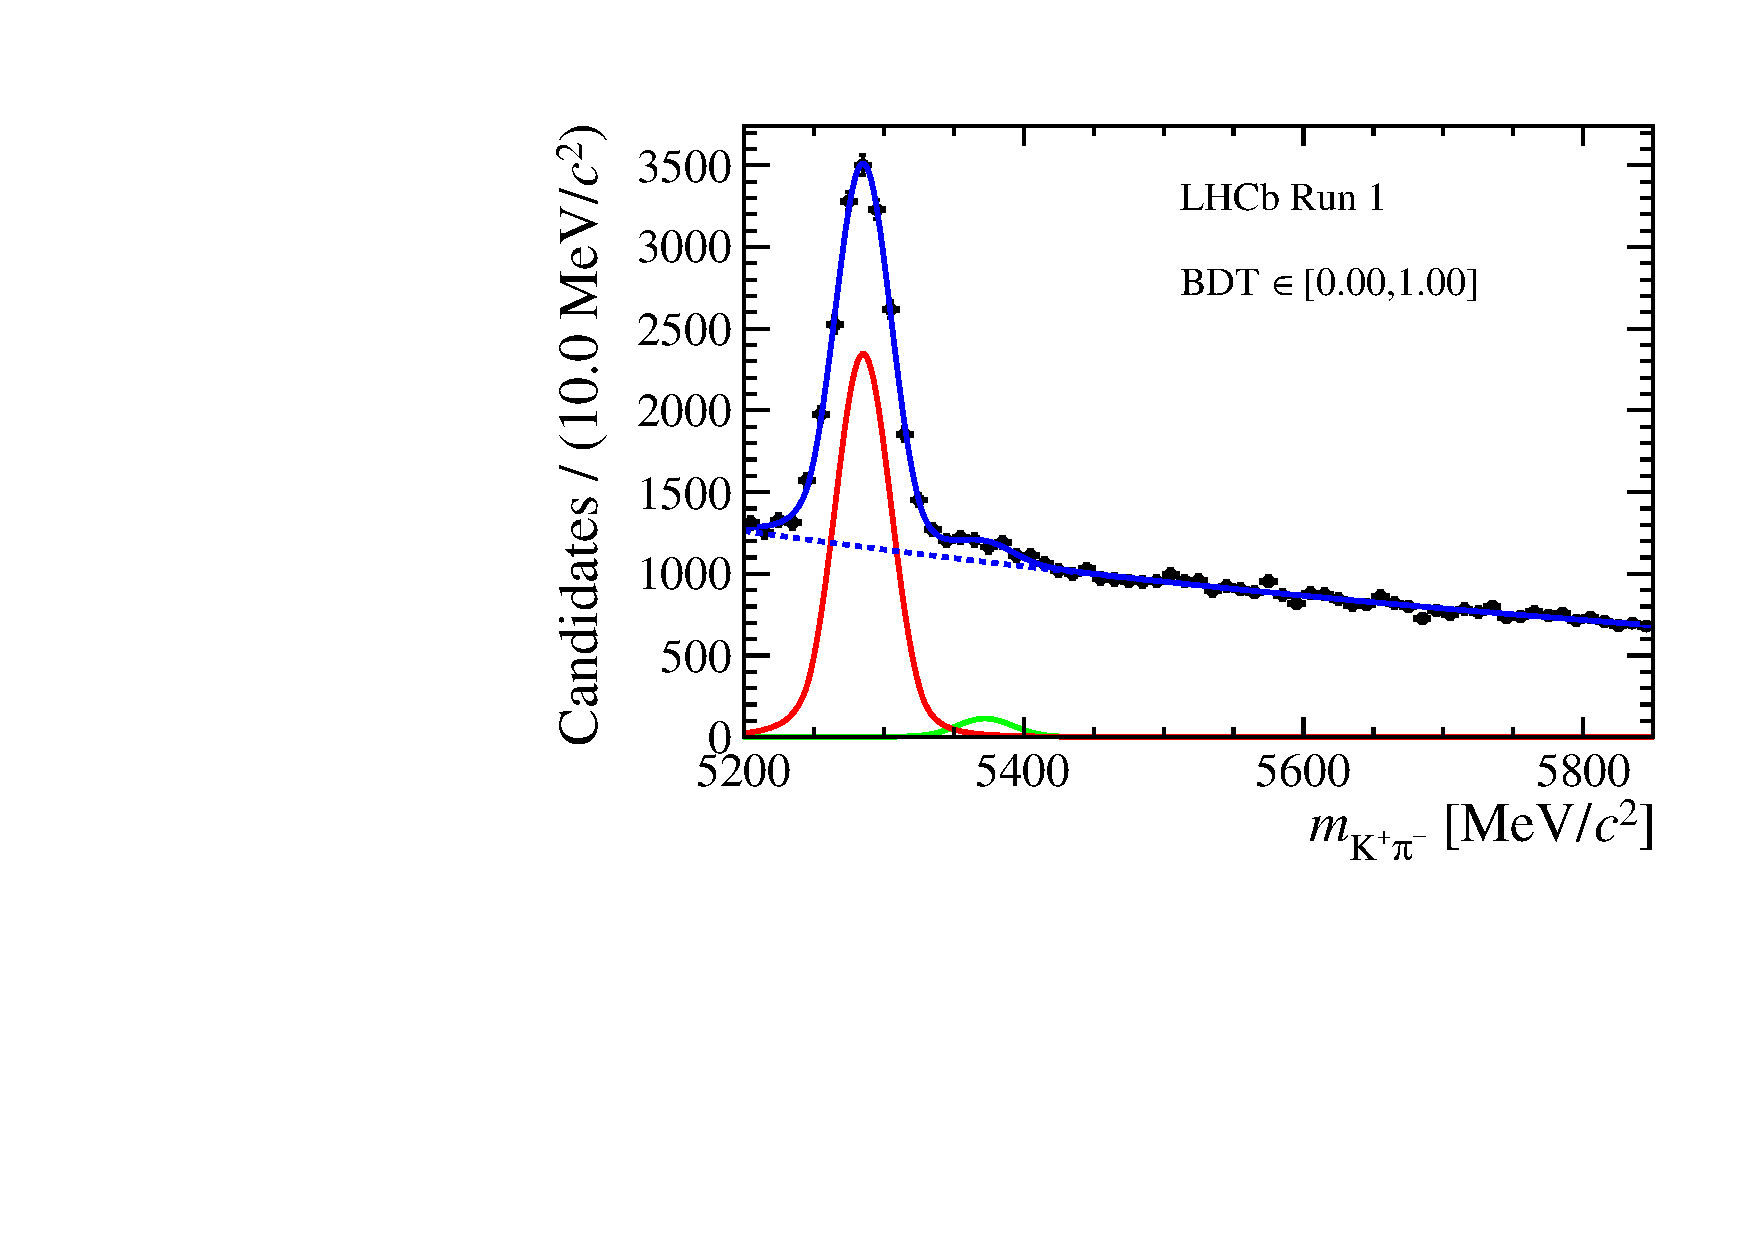
\includegraphics[width=  \textwidth]{./Figs/BFAnalysis/Bd2KPi_mass_RunI_BDTbinNone.pdf}
        %\caption{ }
       % \label{fig:BDTSsig}
    \end{subfigure}
   % ~ %add desired spacing between images, e. g. ~, \quad, \qquad, \hfill etc. 
      %(or a blank line to force the subfigure onto a new line)
    \begin{subfigure}[b]{0.48\textwidth}
       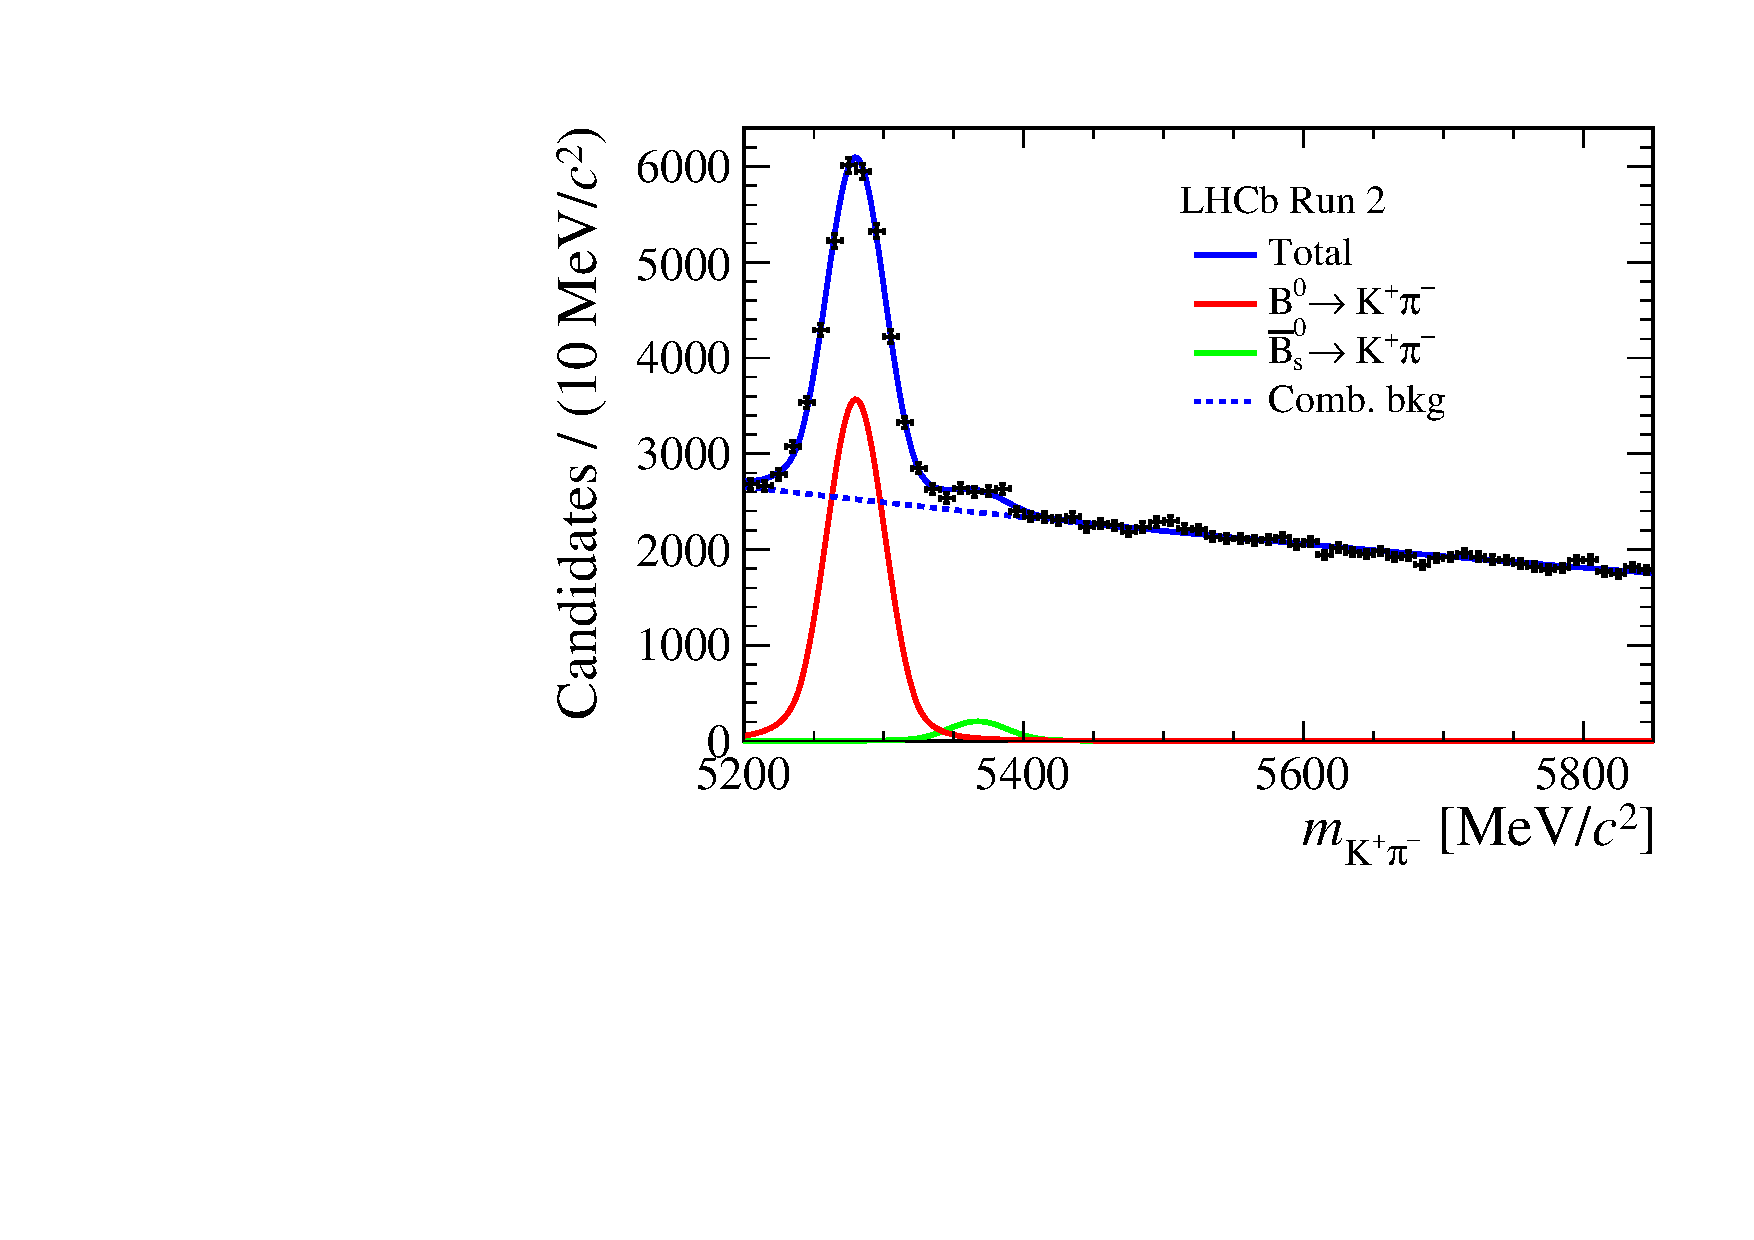
\includegraphics[width=\textwidth]{./Figs/BFAnalysis/Bd2KPi_mass_RunII_BDTbinNone.pdf}
      %  \caption{ }
     %   \label{fig:BDTSbkg}
   \end{subfigure}
    \caption{Mass fit to measure \bdkpi yield for the normalisation for Run 1 (left) and Run 2 (right) data. }
    \label{fig:Bdkpiyield}
\end{figure}



\begin{figure}[htbp]
    \centering
   \begin{subfigure}[b]{0.48\textwidth}
        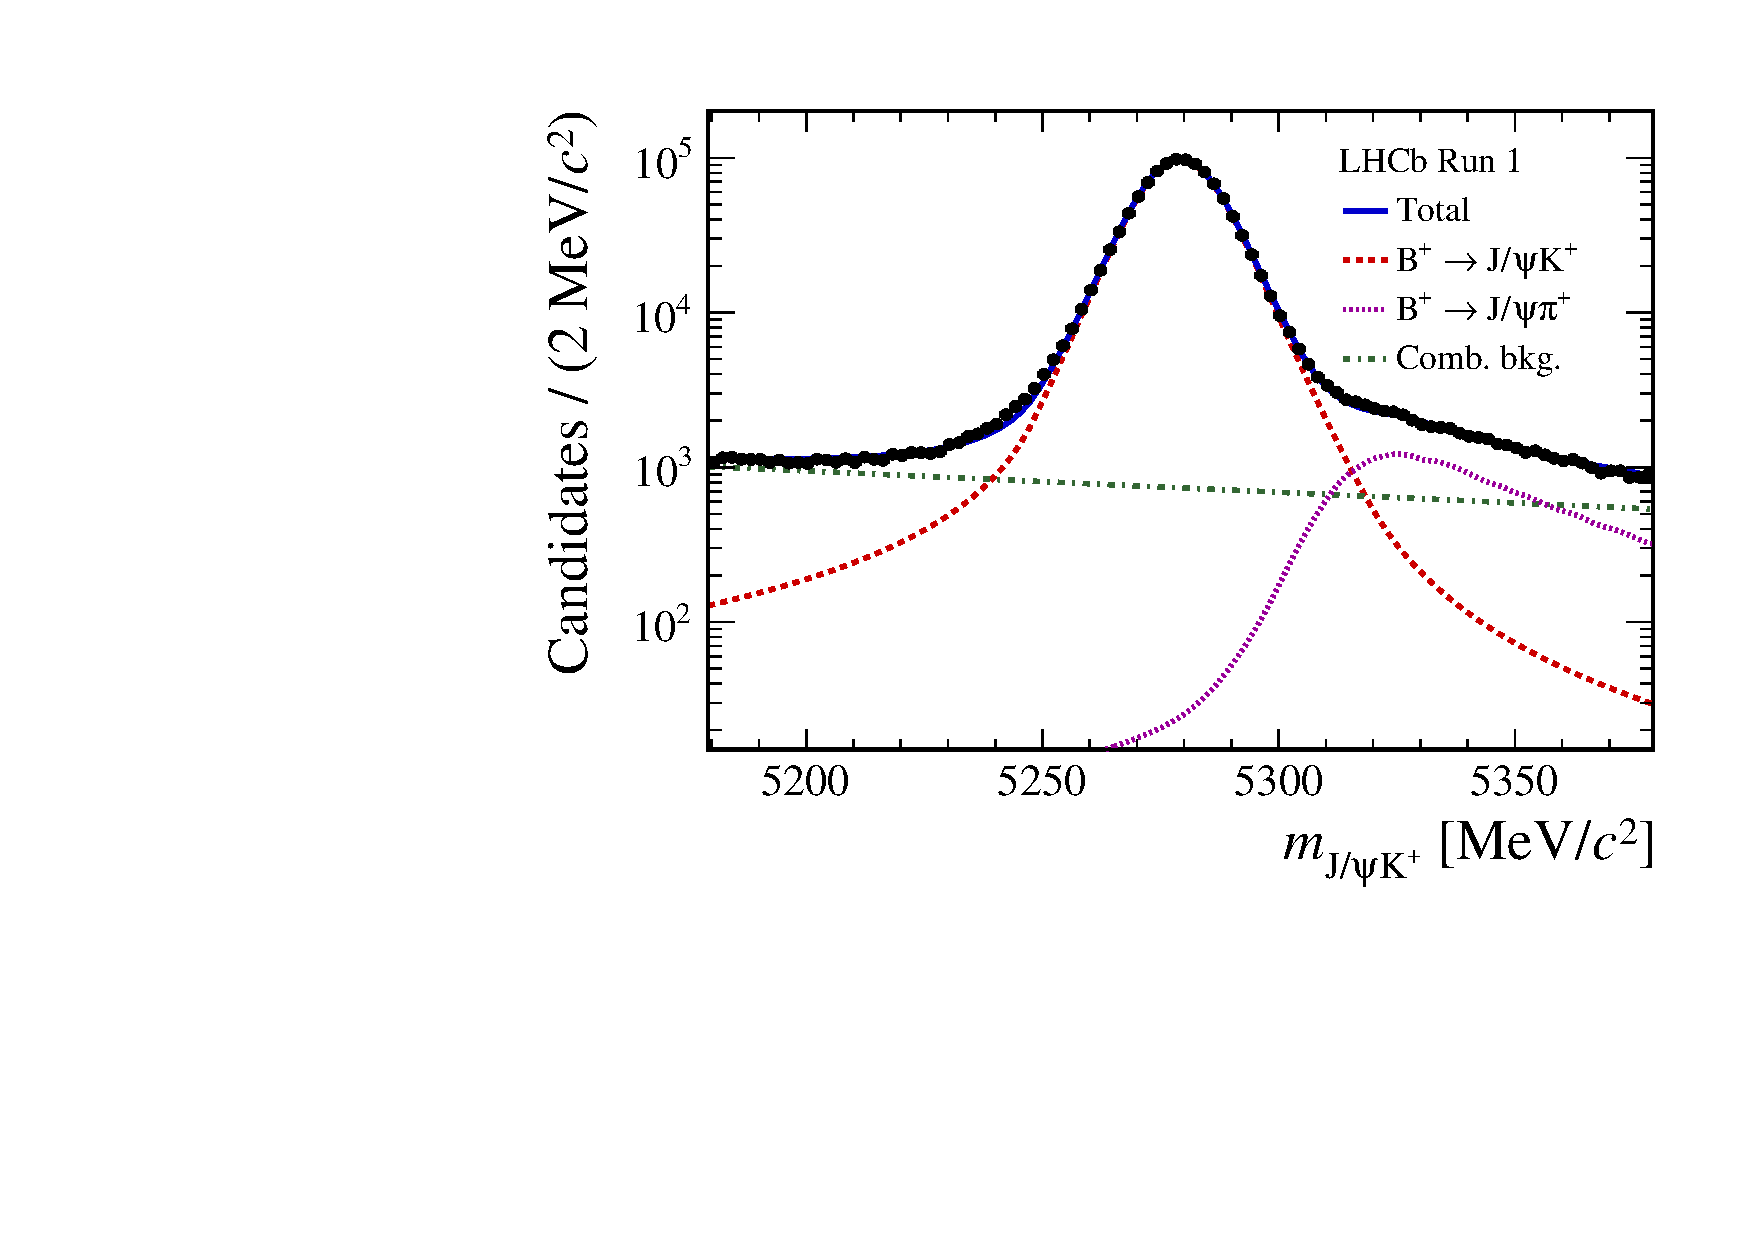
\includegraphics[width=  \textwidth]{./Figs/BFAnalysis/BuJpsiK_Run1.pdf}
        %\caption{ }
       % \label{fig:BDTSsig}
    \end{subfigure}
   % ~ %add desired spacing between images, e. g. ~, \quad, \qquad, \hfill etc. 
      %(or a blank line to force the subfigure onto a new line)
    \begin{subfigure}[b]{0.48\textwidth}
       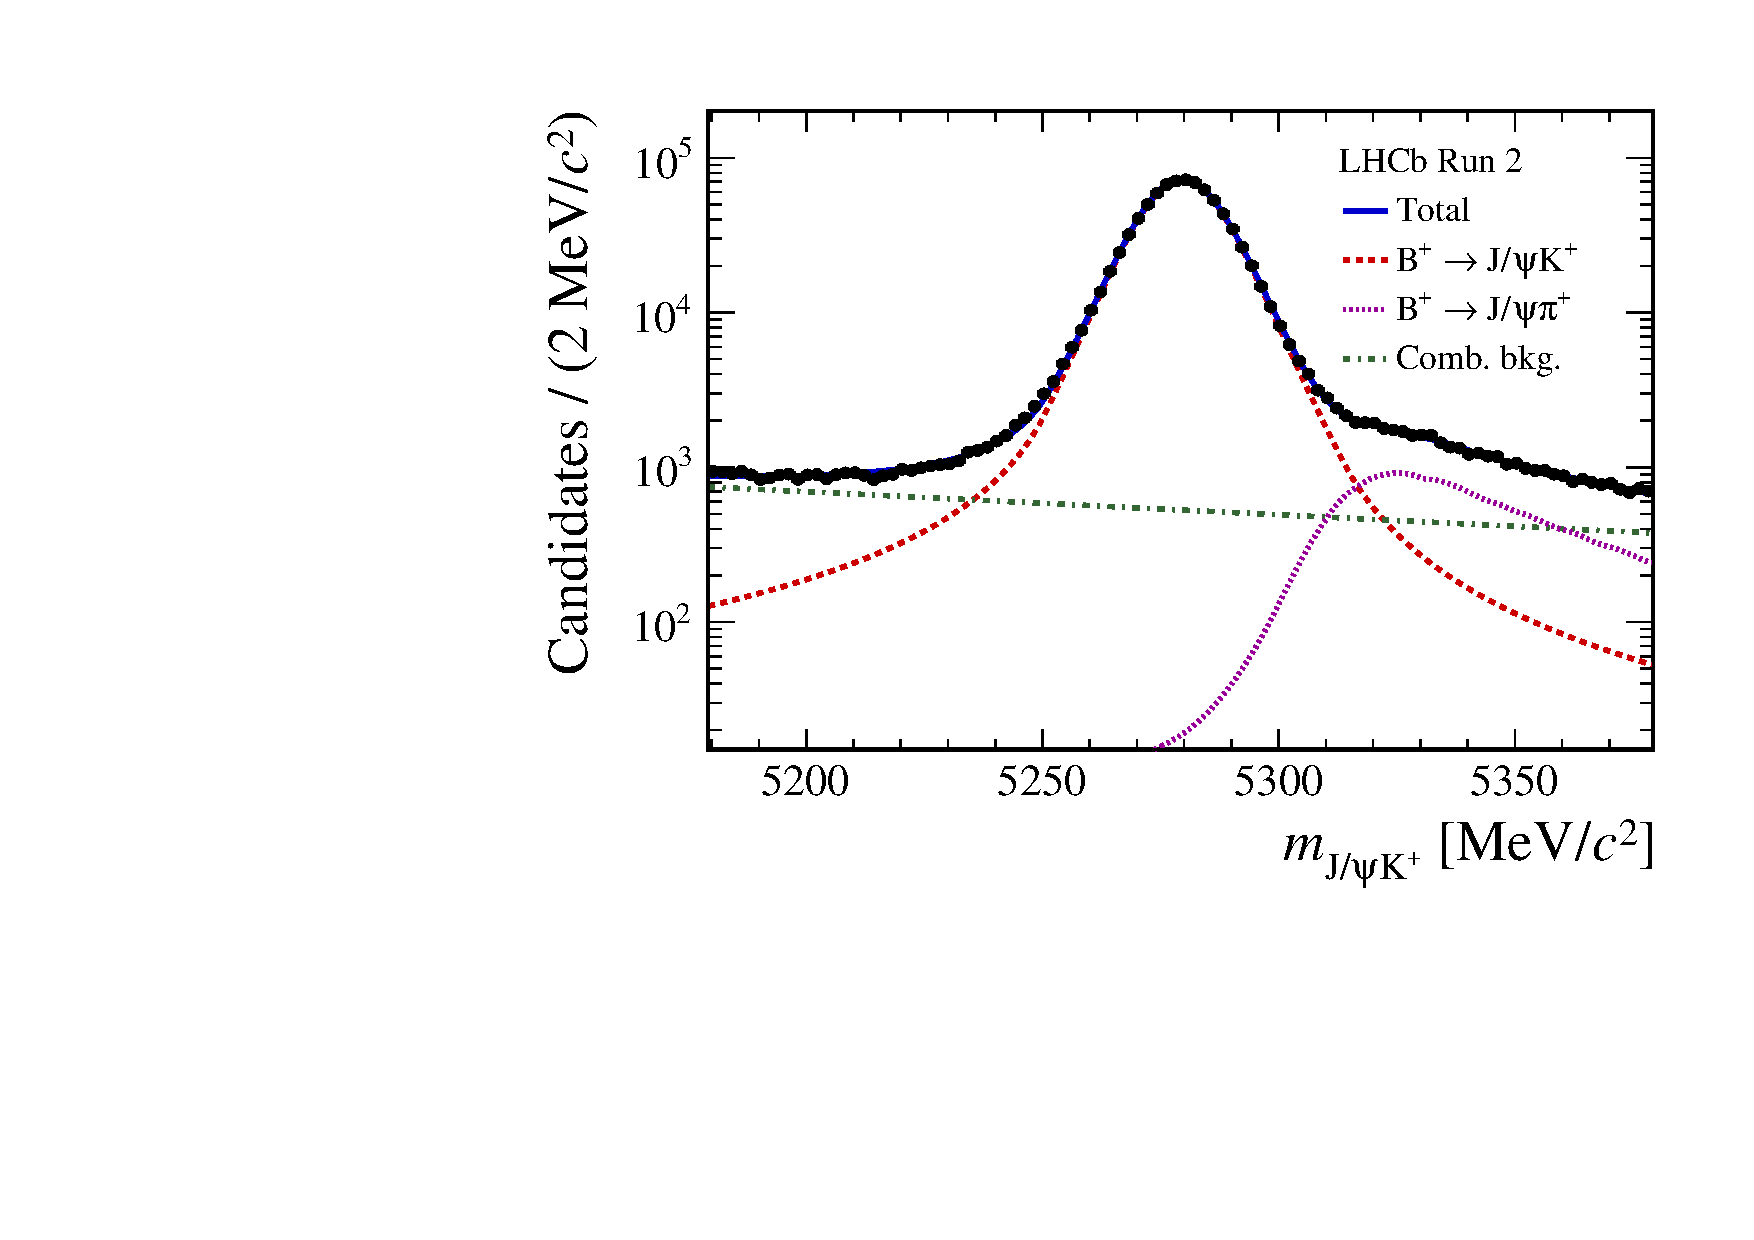
\includegraphics[width=\textwidth]{./Figs/BFAnalysis/BuJpsiK_Run2.pdf}
      %  \caption{ }
     %   \label{fig:BDTSbkg}
   \end{subfigure}
    \caption{ Mass fit to measure \bujpsik yield for the normalisation for Run 1 (left) and Run 2 (right) data.}
    \label{fig:Bujpsikyield}
\end{figure}


\subsection{Efficiency ratio}
The efficiency ratio in equation~\ref{eq:BFnorm} is split into several separate efficiency terms as
\begin{equation}
%\end{split}
\frac{\epsilon_{norm}}{\epsilon_{B^{0}_{(s)} \to \mu^{+} \mu^{-}}}  =  \frac{\epsilon^{Acc}_{norm}}{\epsilon^{Acc}_{B^{0}_{(s)} \to \mu^{+} \mu^{-}}} \cdot \frac{\epsilon^{RecSel|Acc}_{norm}}{\epsilon^{RecSel|Acc}_{B^{0}_{(s)} \to \mu^{+} \mu^{-}}} \cdot \frac{\epsilon^{Trig|RecSel}_{norm}}{\epsilon^{Trig|RecSel}_{B^{0}_{(s)} \to \mu^{+} \mu^{-}}}
%\end{split}
\label{eq:BFnormDetailed}
\end{equation}
for the detector acceptance, $\epsilon^{Acc}$, reconstruction and selection efficiencies, $epsilon^{RecSel|Acc}$, and the trigger efficiency, $\epsilon^{Trig|RecSel}$. 

The detector acceptance efficiency gives the efficiency for the decay products to be within the LHCb detector acceptance. This efficiency is evaluated on simulated decays to for decay products that fall within the range [10,400] mrad. The range is chosen to be slightly larger than the detector acceptance so that particles recover by the magnetic field are included. To keep this efficiency similar for \bmumu and \bdkpi decays, the hadrons from \bdkpi are required to be within the muon detector acceptance. 

The reconstruction and selection efficiencies are calculated as the reconstruction efficiency of decays that are within the detector acceptance and the selection efficiency of reconstructed decays. The selection and reconstruction efficiencies are evaluated from a combination of information from data and simulated decays to ensure accurate selection efficiency ratios. Similar to the \bsmumu BDT \pdf a correction is applied for the lifetime used in simulated \bsmumu decays assuming \ADG = +1. 

The trigger efficiencies for decays passing the reconstruction and selection are evaluated for each decay by data driven methods as descried in~\ref{}. 

The efficiencies are calculated for \bsmumu, \bdmumu, \bdkpi and \bujpsik separately to account for difference in the decays and kinematics. The ratio of efficiencies between signal and normalisation channels in the normalisation parameters ensures that systematic uncertainties arising from the use of simulated decays cancel out and will not effect the precision of the \bmumu branching fractions.

\subsection{Hadronisation factors}

The normalisation factors depend on hadronisation factors, $f_{u}, f_{s}, f_{d}$, that give the probability of a $b$ or $\bar{b}$ quark to form a particular $B^{+}$, \bs or \bd, respectively. The hadronisation factors $f_{d}$ and $f_{u}$ are equal therefore the \bdmumu branching fraction does not depend on any hadronisation factors. For the \bsmumu the ratio $f_{s}/f_{d}$ is used in the normalisation, since $f_{d} = f_{u}$. This ratio was measured at LHCb for $pp$ collisions at $\sqrt{s}$ = 7 TeV, and it is used for the different LHC $\sqrt{s}$ energies. However for Run 2 the $f_{s}/f_{d}$ ratio must be modified for the small observed relative production difference. 
The uncertainty on the hadronisation factor ratio contributes the largest uncertainty to the \bsmumu branching fraction. Alternatively the \bsmumu decay could be normalised using a different \bs decay however the precision of the measured branching fractions and abundance of \bs decays, such as \bsjpsiphi, are not high enough at present to provide a lower overall uncertainty on the normalisation factors than the $f_{s}/f_{d}$ ratio.

\subsection{Normalisation parameters}

The yields, efficiencies and hadronisation factors are combined to produce separate normalisation factors for each year of data taking and each normalisation channel. The yearly normalisation factors are combined for each channel using to produce the normalisation factors for Run 1 and for Run 2 taking into account correlations between the parameters. A weighted average of the normalisation factors for \bdkpi and \bujpsiK is used to produce the overall normalisation factors for Run 1 and Run 2 as shown in Table~\ref{tab:normparams}.

\begin{table}[htbp]
\begin{center}
\begin{tabular}{lcc}
\hline
Normalisation Paramters & Run 1 & Run 2 \\ \hline
$\alpha_{d} \times 10^{11}$ & 2.877 $\pm$ 0.101 & 3.521 $\pm$ 0.155 \\ %Why are they so differe  
$\alpha_{s} \times 10^{10}$ & 1.071 $\pm$ 0.072 & 1.306$ \pm$ 0.095 \\
\hline
\end{tabular}
\vspace{0.7cm}
\caption{Noramlisation parameters for \bsmumu and \bdmumu for Run 1 and Run 2.}
\label{tab:normparams}
\end{center}
\end{table}


\section{Results}
\label{sec:BFResults}

As described earlier in Section~\ref{sec:BFAnalysisStrategy} the \bsmumu and \bmumu branching fractions are measured by a simultaneous maximum likelihood fit to the dimuon invariant mass of the Run 1 and Run 2 data sets, each divided into four BDT bins. 

In the fit the mass \pdfs and fraction of \bmumu decays in each BDT bin are constrained within Gaussian limits using the expected values and uncertainties. The yield of the combinatorial background is left free in the fit in each BDT bin and the slope of the mass distribution is constrained to have the same value across all bins for each data set. The yields of the backgrounds from \bhh, \bdpimunu, \bsKmunu, \bpimumu, \bdpimumu and \bcjpsimunu decays in each BDT bin are constrained around the expected values, similarly to the signal fractions but the mass shapes are fixed in the fit.

The branching fraction results from the fit are;

\begin{equation}
%\begin{align}
\begin{split}
  \mathcal{B}(B^{0}_{s} \to \mu^{+} \mu^{-}) &= (2.8 \pm 0.6) \times 10^{-9} \\
  \mathcal{B}(B^{0} \to \mu^{+} \mu^{-}) &= (1.6^{+1.1}_{-0.9})    \times 10^{-10} 
%\end{align}
\end{split}
\label{eq:BFresults}
\end{equation}

Figure~\ref{fig:BFfit} shows the fit results for \bmumu candidates in the 4 BDT bins for both Run 1 and Run 2 data and Figure~\ref{fig:contour} the 2-dimensional likelihood profile for the \bdmumu and \bsmumu branching fraction measurements.
The statistical significance of the \bsmumu signal is 7.9 $\sigma$ which is the first single experiment observation of the \bsmumu decay. While the significance of the \bdmumu signal is less at 1.9$\sigma$, therefore the CLs method is used to place an upper limit on the branching fraction of $\mathcal{B}$(\bdmumu)$ < 3.4 \times 10^{-10}$  at the 95~$\%$ confidence level.

The quoted \bsmumu branching fraction assumes the SM value for \ADG, applying the corrections detailed in Section~\ref{sec:ADGBDTcorrections} for \ADG values of 0 and -1 shift the central value of $\mathcal{B}$(\bsmumu) by 4.6 $\%$ and 10.9 $\%$, respectively. All results are consistent with the predictions of the Standard Model.



%\begin{figure}[htbp] %Put in the summary.
%    \centering
%        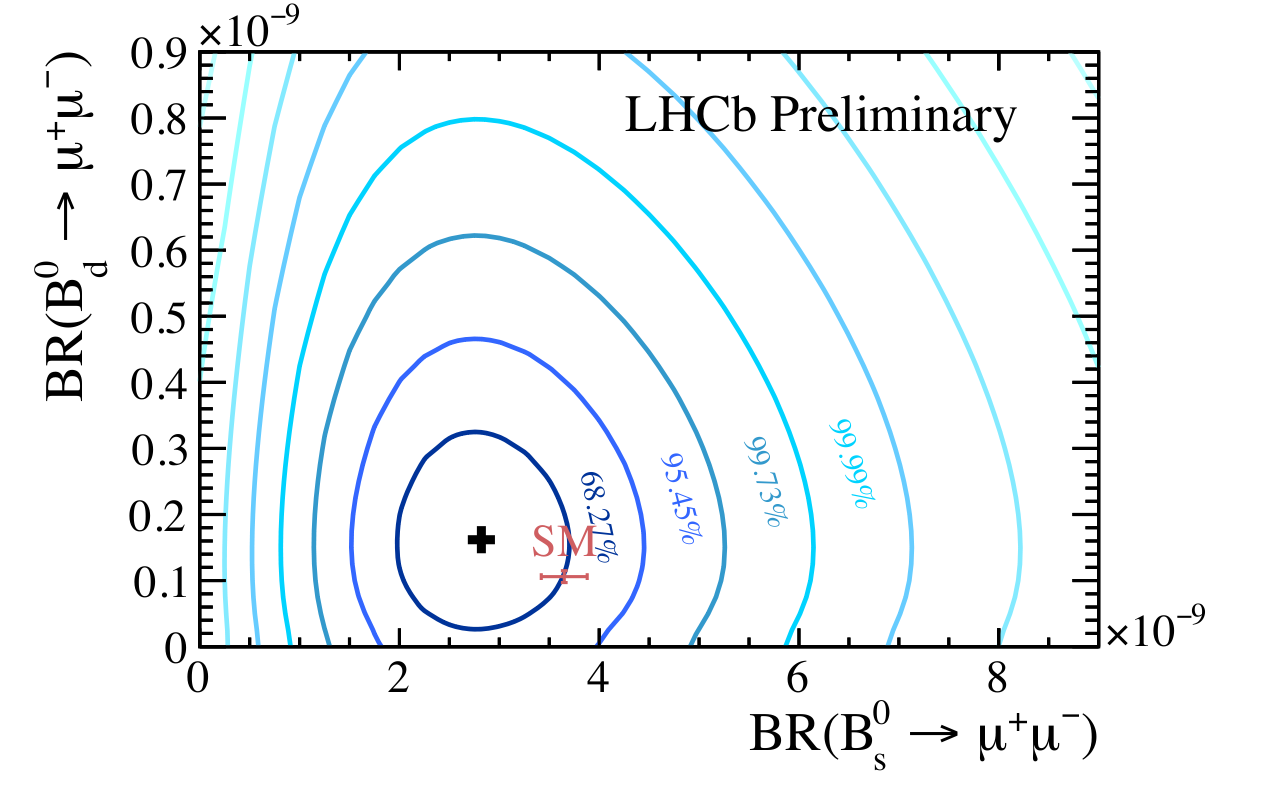
\includegraphics[width= 0.8 \textwidth]{./Figs/BFAnalysis/2D_contour_plot.png}
%      \caption{\bdmumu and \bsmumu 2-dimesnional likelihood plot for the simultaneous branching fraction fit to Run 1 and Run 2 data. }
%    \label{fig:contour}
%\end{figure}


\begin{figure}[htbp]
    \centering
    \begin{subfigure}[b]{0.48\textwidth}
        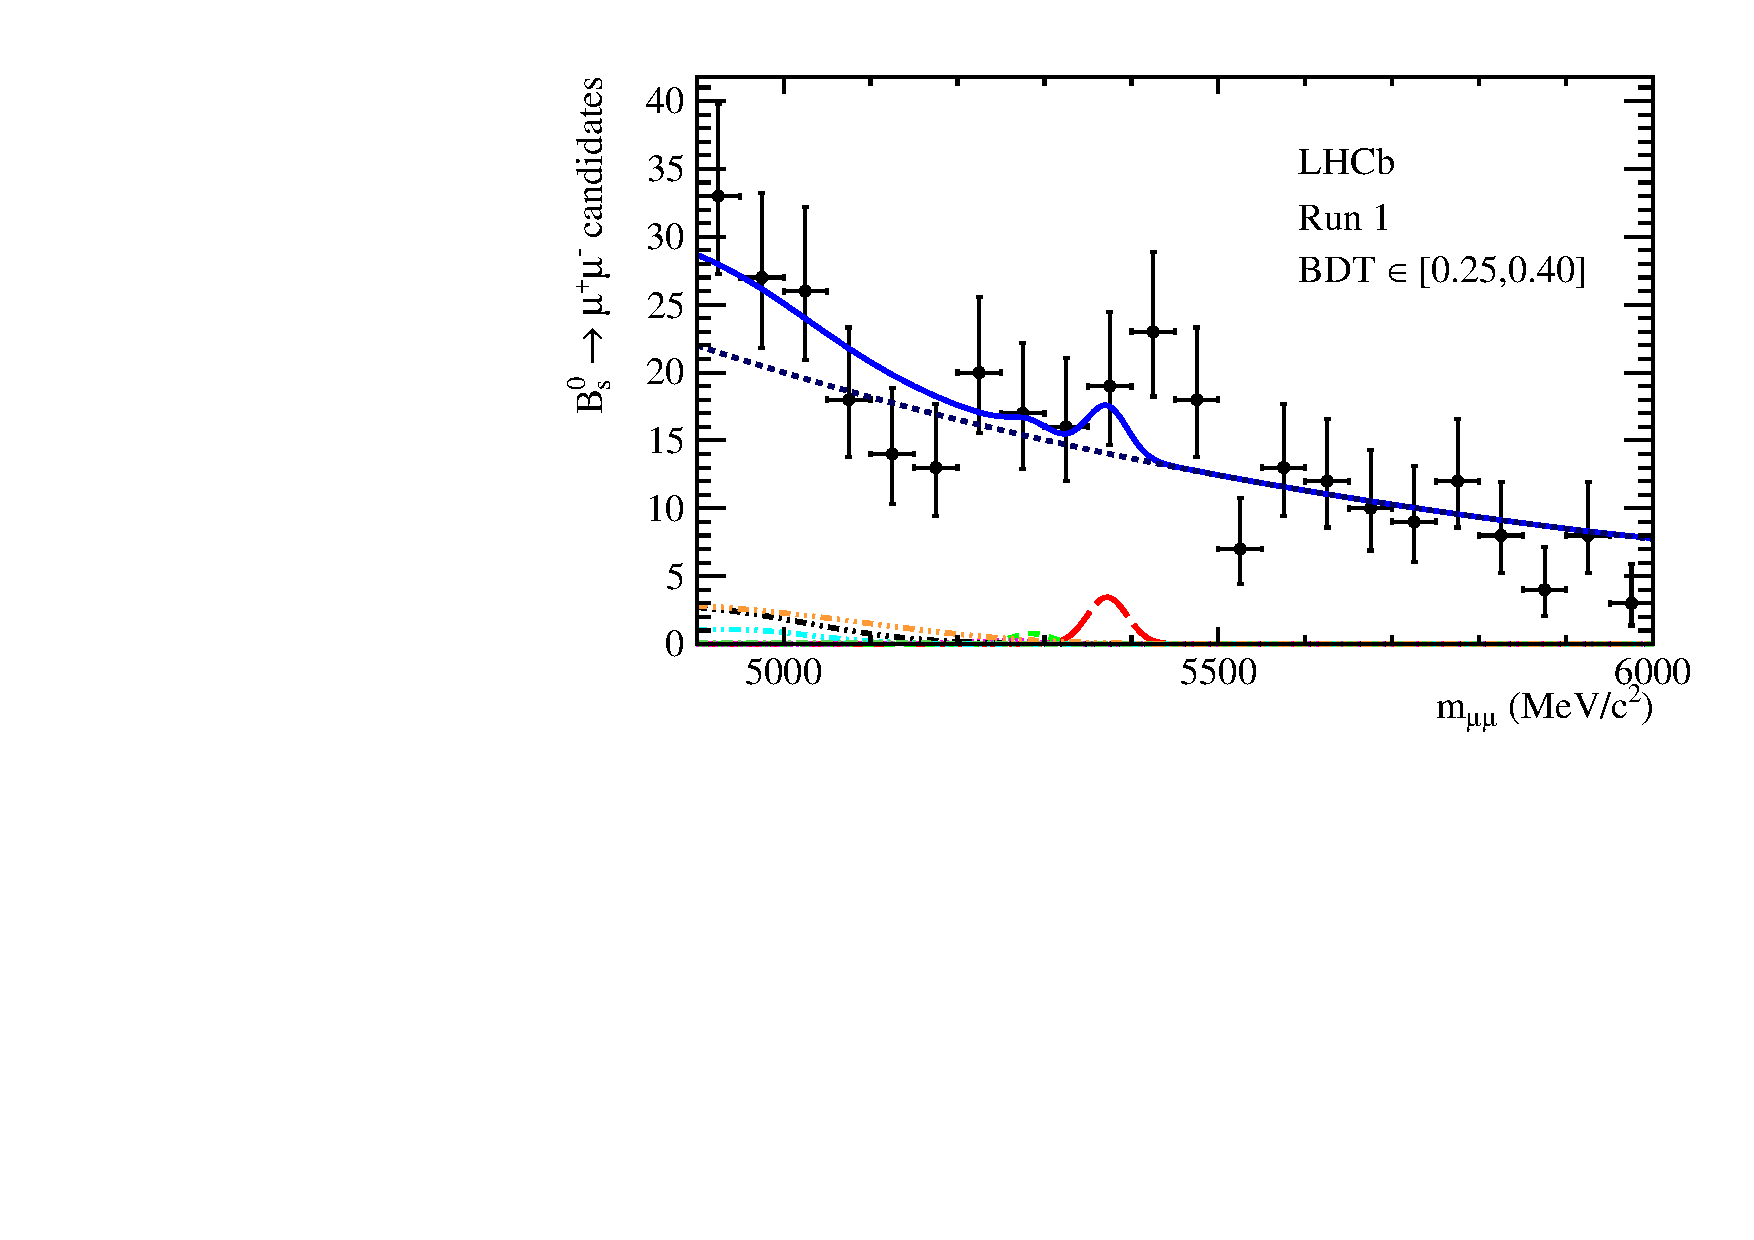
\includegraphics[width=\textwidth]{./Figs/BFAnalysis/Bsmumu_Fit_Run1_bin2.pdf}
    \end{subfigure}
    ~ %add desired spacing between images, e. g. ~, \quad, \qquad, \hfill etc. 
      %(or a blank line to force the subfigure onto a new line)
    \begin{subfigure}[b]{0.48\textwidth}
       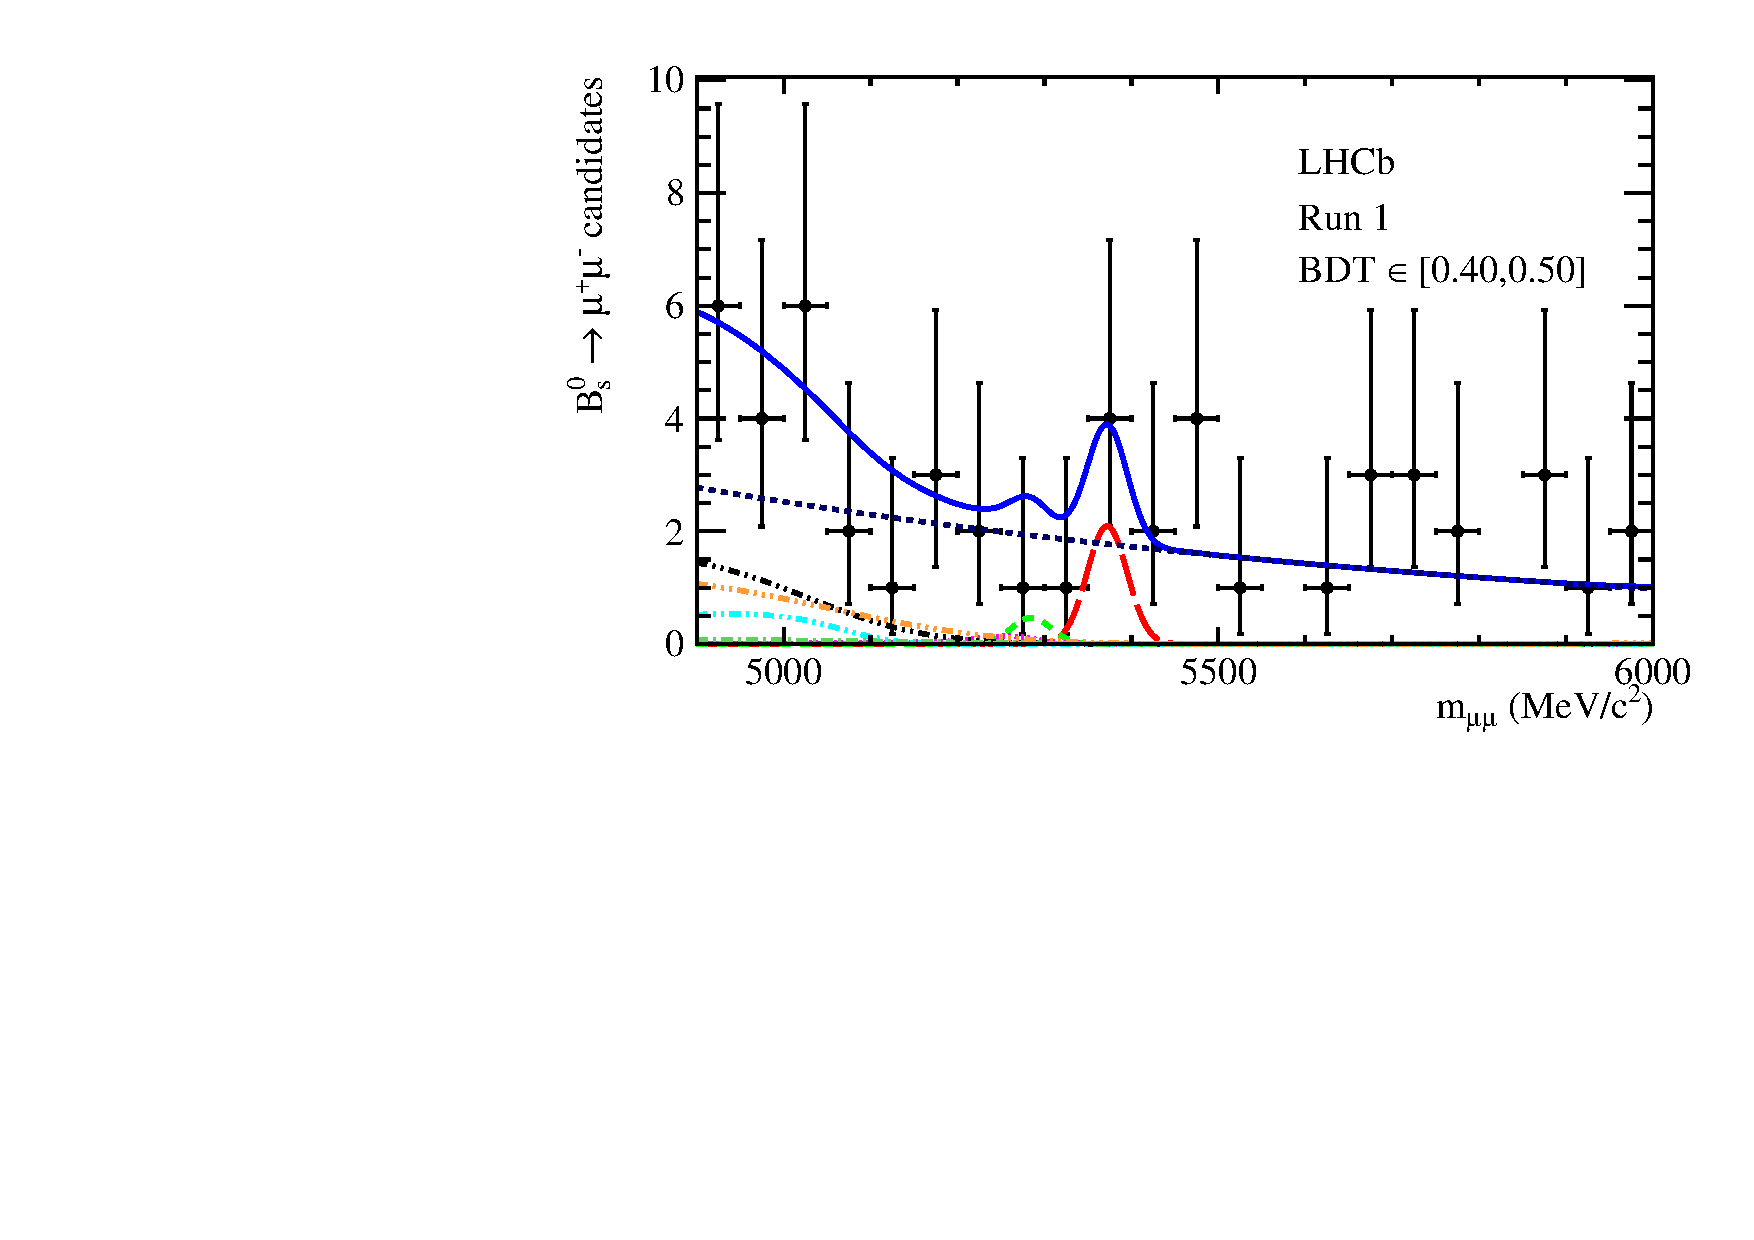
\includegraphics[width=\textwidth]{./Figs/BFAnalysis/Bsmumu_Fit_Run1_bin3.pdf}
    \end{subfigure}
    \begin{subfigure}[b]{0.48\textwidth}
        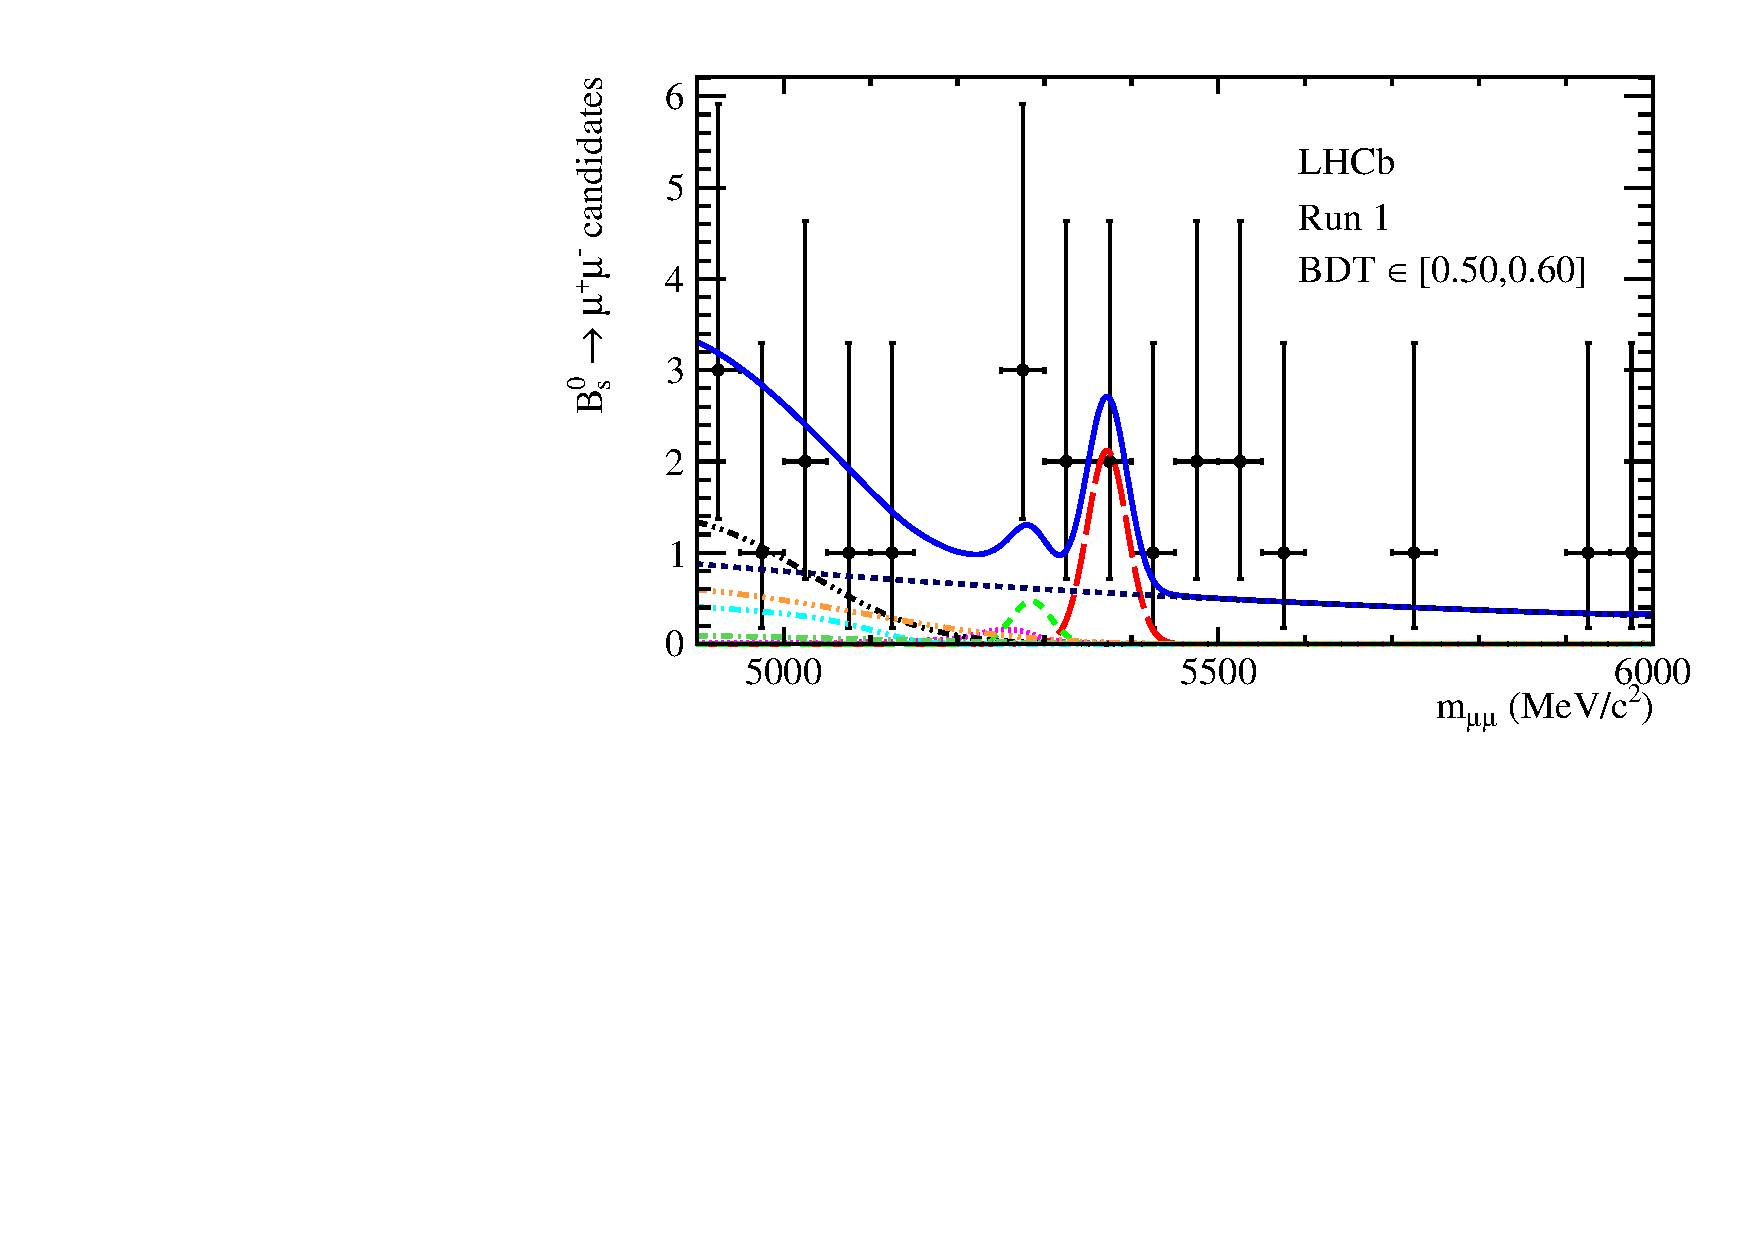
\includegraphics[width=\textwidth]{./Figs/BFAnalysis/Bsmumu_Fit_Run1_bin4.pdf}
    \end{subfigure}
    ~ %add desired spacing between images, e. g. ~, \quad, \qquad, \hfill etc. 
      %(or a blank line to force the subfigure onto a new line)
    \begin{subfigure}[b]{0.48\textwidth}
       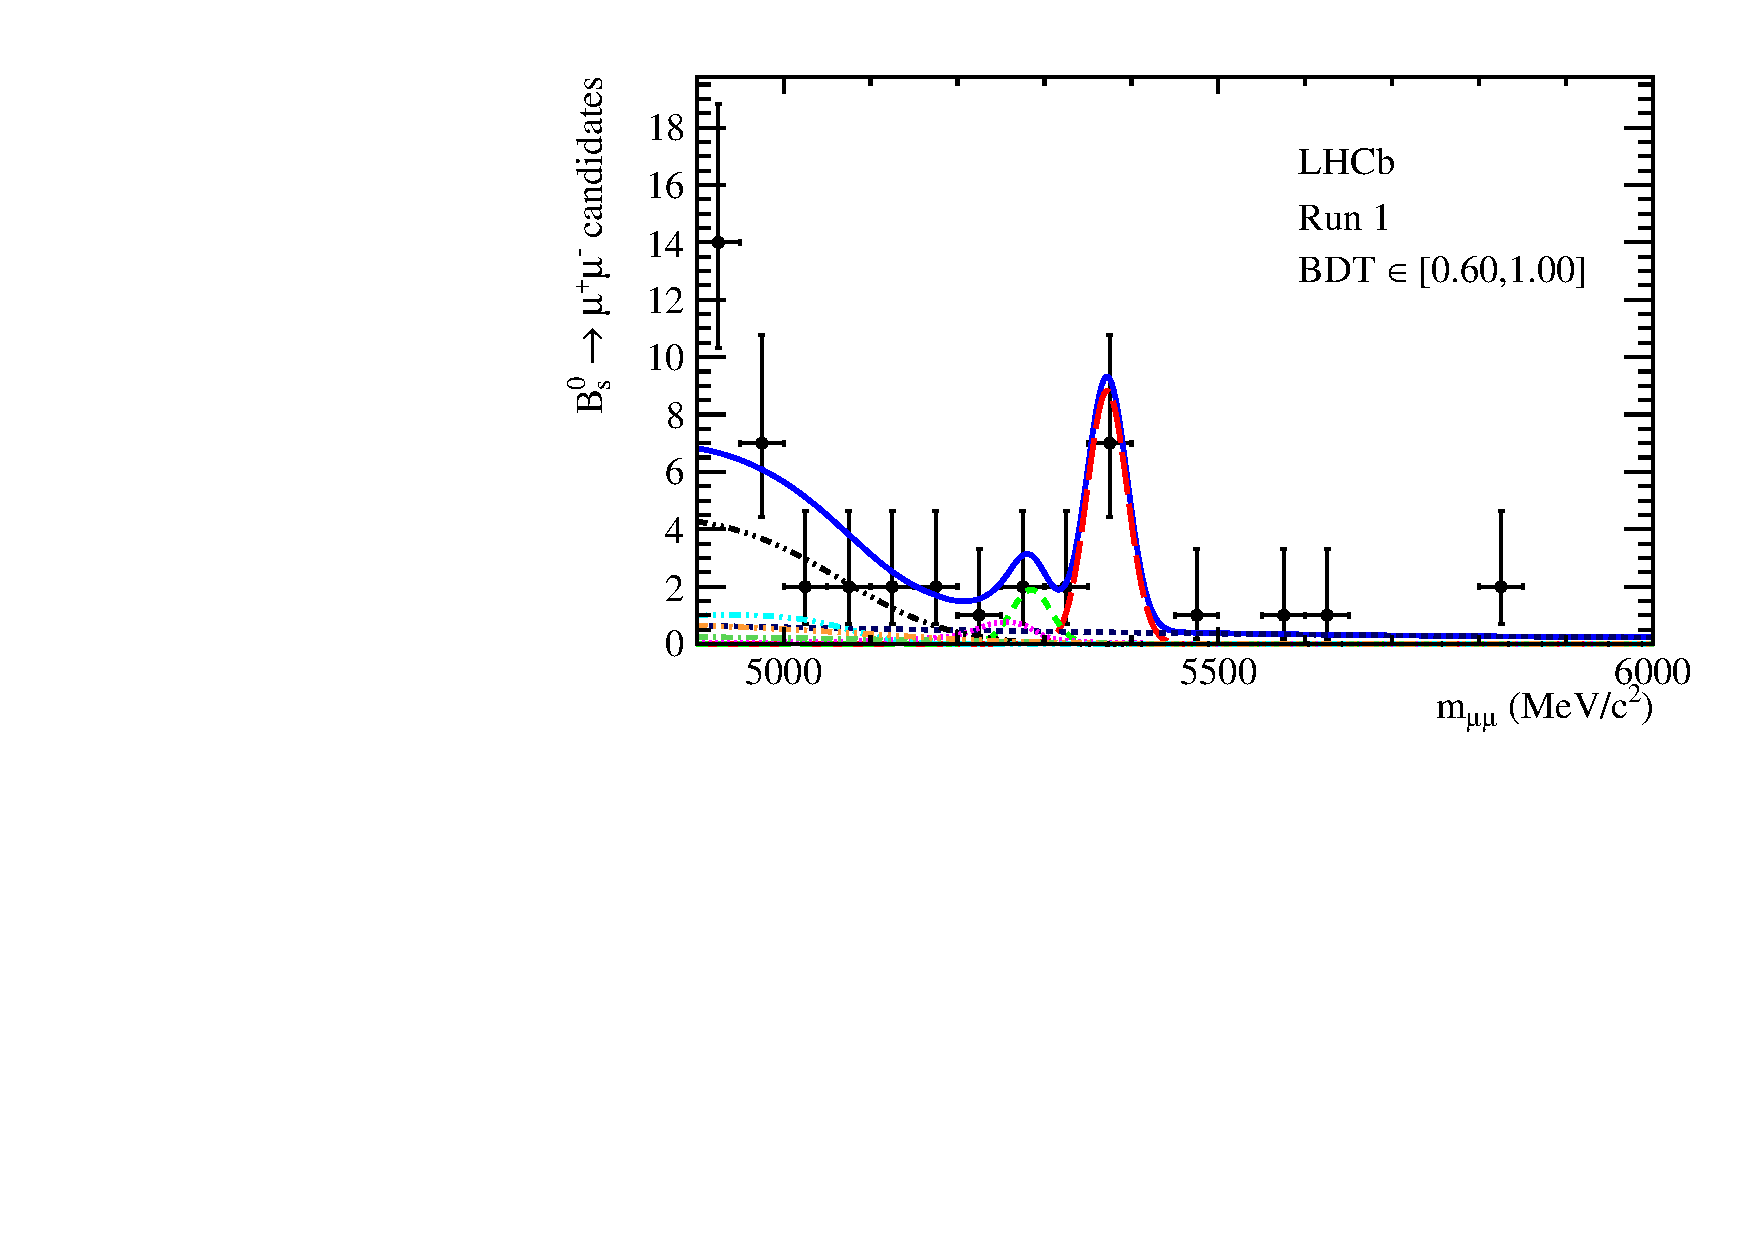
\includegraphics[width=\textwidth]{./Figs/BFAnalysis/Bsmumu_Fit_Run1_bin5.pdf}
    \end{subfigure}

    \qquad

    \begin{subfigure}[b]{0.48\textwidth}
        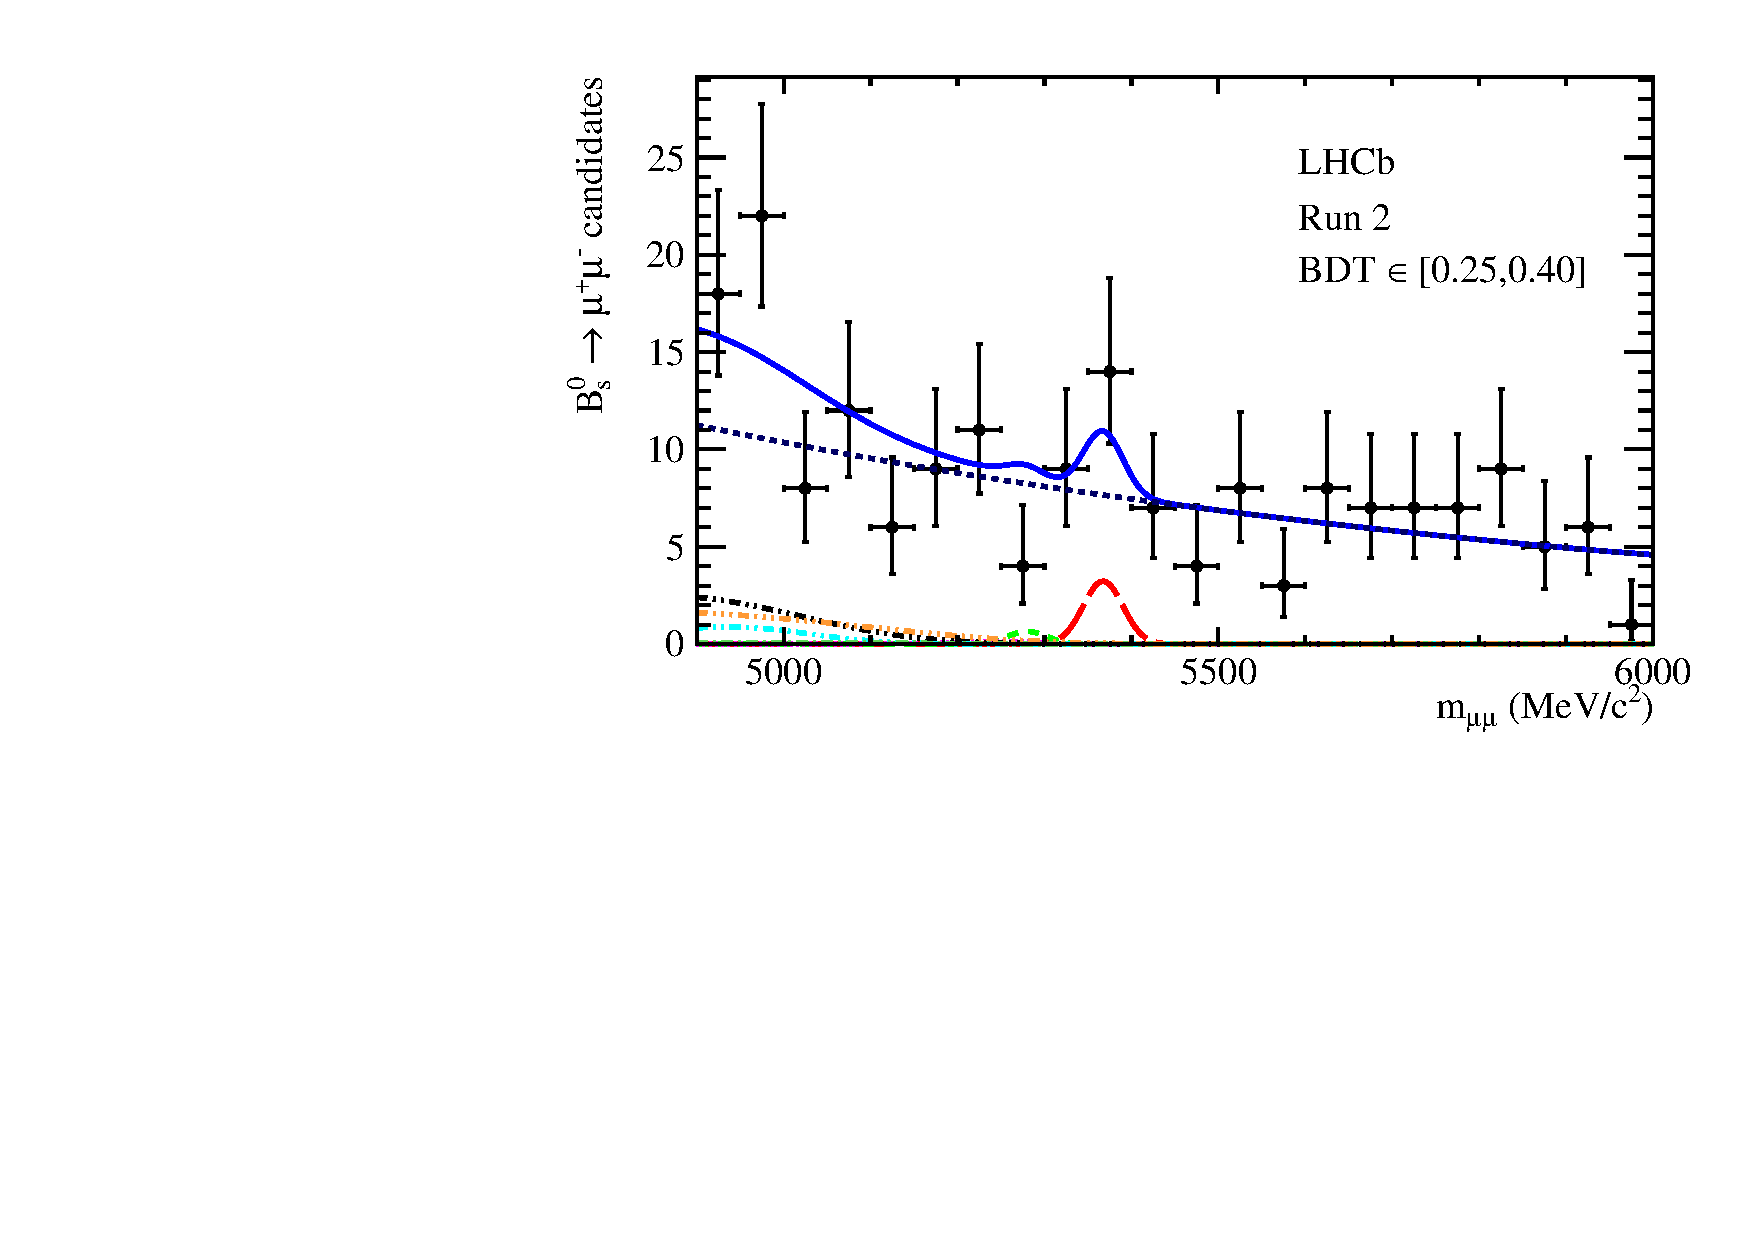
\includegraphics[width=\textwidth]{./Figs/BFAnalysis/Bsmumu_Fit_Run2_bin2.pdf}
    \end{subfigure}
    ~ %add desired spacing between images, e. g. ~, \quad, \qquad, \hfill etc. 
      %(or a blank line to force the subfigure onto a new line)
    \begin{subfigure}[b]{0.48\textwidth}
       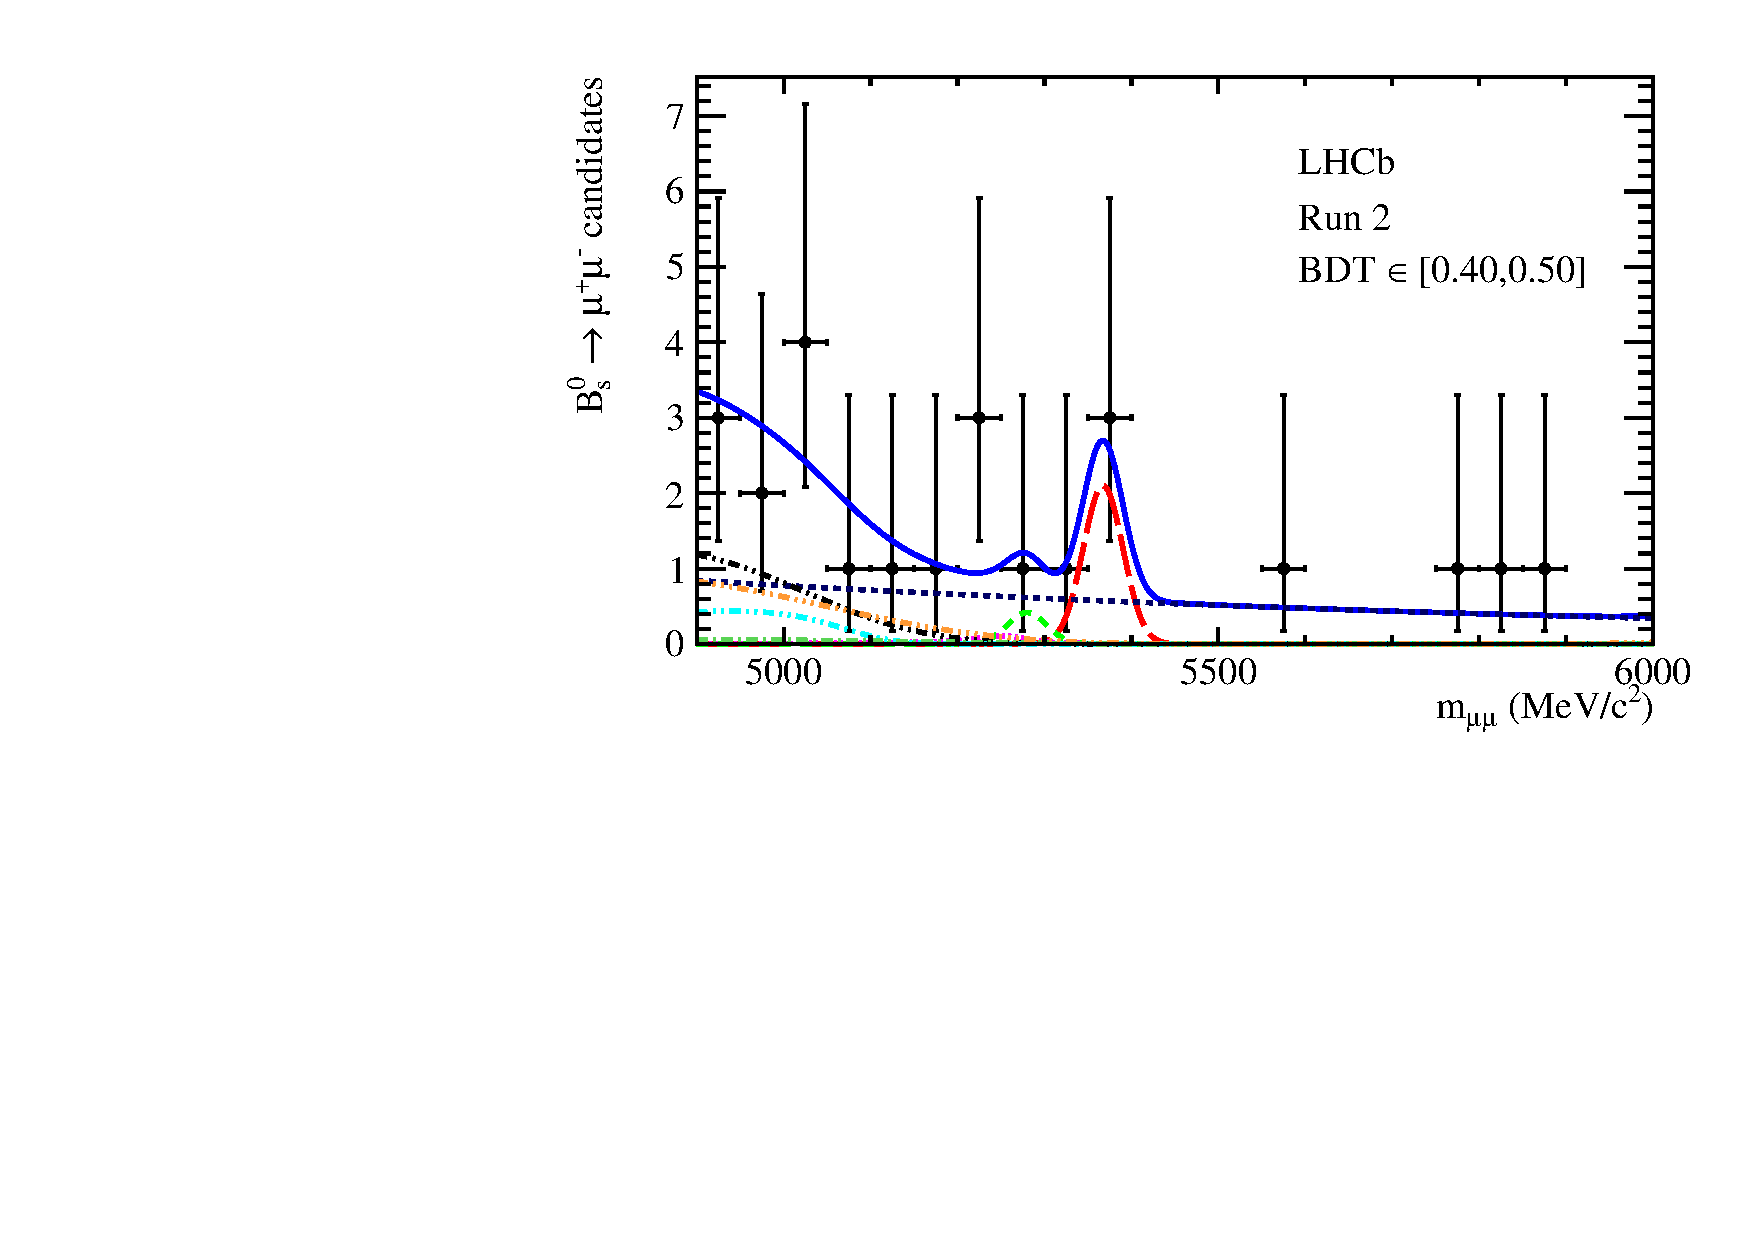
\includegraphics[width=\textwidth]{./Figs/BFAnalysis/Bsmumu_Fit_Run2_bin3.pdf}
    \end{subfigure}
    \begin{subfigure}[b]{0.48\textwidth}
        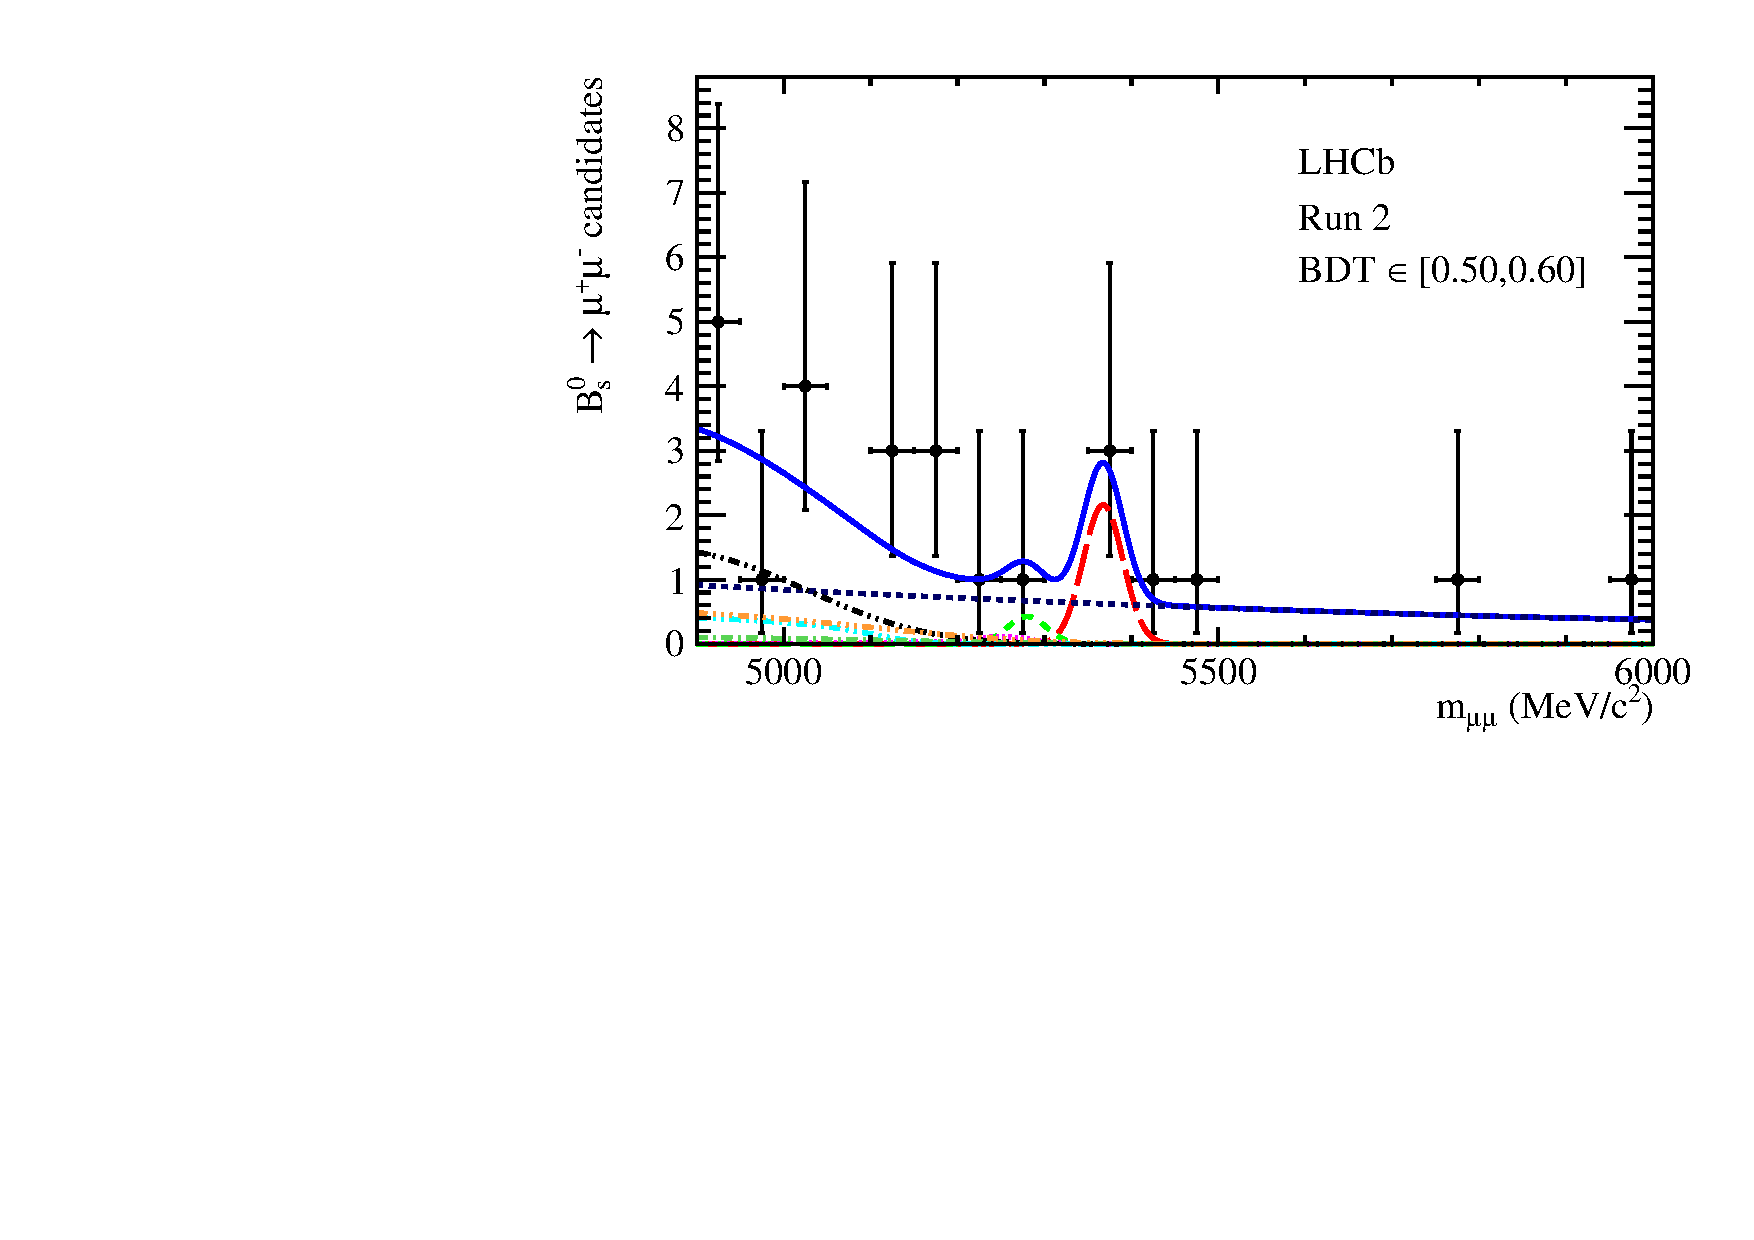
\includegraphics[width=\textwidth]{./Figs/BFAnalysis/Bsmumu_Fit_Run2_bin4.pdf}
    \end{subfigure}
    ~ %add desired spacing between images, e. g. ~, \quad, \qquad, \hfill etc. 
      %(or a blank line to force the subfigure onto a new line)
    \begin{subfigure}[b]{0.48\textwidth}
       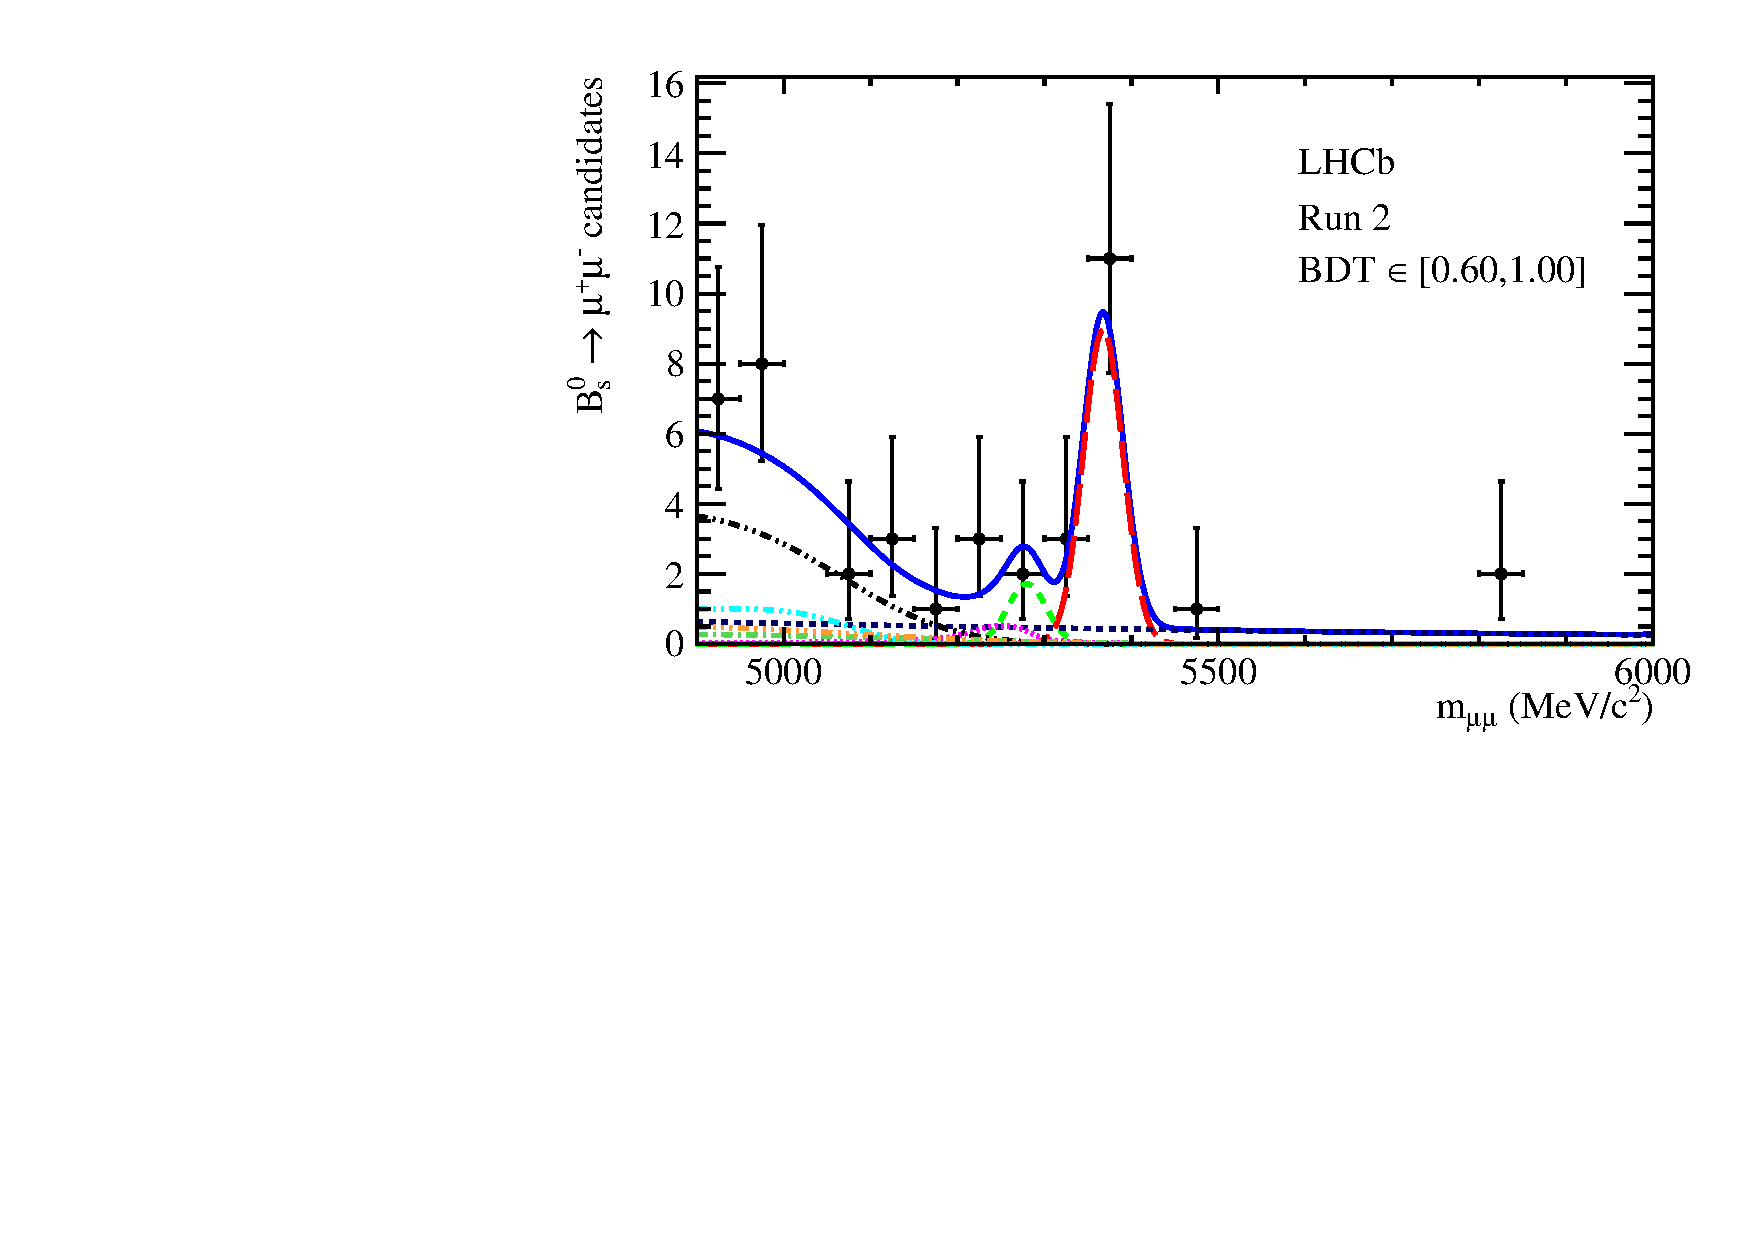
\includegraphics[width=\textwidth]{./Figs/BFAnalysis/Bsmumu_Fit_Run2_bin5.pdf}
    \end{subfigure}

    \begin{subfigure}[b]{0.3\textwidth}
       \includegraphics[width=\textwidth]{./Figs/BFAnalysis/legendA.pdf}
    \end{subfigure}
    ~
    \begin{subfigure}[b]{0.3\textwidth}
       \includegraphics[width=\textwidth]{./Figs/BFAnalysis/legendB.pdf}
    \end{subfigure}
    \caption{Mass distribution in BDT bins for selected \bsmumu and \bdmumu candidates with the fit overlaid for Run 1 and Run 2 data. The fit includes components for \bdmumu, \bsmumu, combinatorial backgrounds, mis-identified \bhh decays and backgrounds from semi-leptonic decays. {\it Needs to be updated for new tail parameters.}}
    \label{fig:BFfit}
\end{figure}



%{\bf some things I should learn about the BF analysis or I think I should mention. The correlation, orlack ok, between the mass and BDT output. The cascade B decays that are removed by the lower 4900 mass cut (Alessio) and also the decays that contribute to CBG (Siim).}

%{\it prehaps put plots and numbers in the appendix??}
